\documentclass[man,floatsintext]{apa6}
\usepackage{lmodern}
\usepackage{amssymb,amsmath}
\usepackage{ifxetex,ifluatex}
\usepackage{fixltx2e} % provides \textsubscript
\ifnum 0\ifxetex 1\fi\ifluatex 1\fi=0 % if pdftex
  \usepackage[T1]{fontenc}
  \usepackage[utf8]{inputenc}
\else % if luatex or xelatex
  \ifxetex
    \usepackage{mathspec}
  \else
    \usepackage{fontspec}
  \fi
  \defaultfontfeatures{Ligatures=TeX,Scale=MatchLowercase}
\fi
% use upquote if available, for straight quotes in verbatim environments
\IfFileExists{upquote.sty}{\usepackage{upquote}}{}
% use microtype if available
\IfFileExists{microtype.sty}{%
\usepackage{microtype}
\UseMicrotypeSet[protrusion]{basicmath} % disable protrusion for tt fonts
}{}
\usepackage{hyperref}
\hypersetup{unicode=true,
            pdftitle={Seeking social information during language comprehension and word learning},
            pdfauthor={Kyle MacDonald, Elizabeth Swanson, \& Michael C. Frank},
            pdfborder={0 0 0},
            breaklinks=true}
\urlstyle{same}  % don't use monospace font for urls
\usepackage{graphicx,grffile}
\makeatletter
\def\maxwidth{\ifdim\Gin@nat@width>\linewidth\linewidth\else\Gin@nat@width\fi}
\def\maxheight{\ifdim\Gin@nat@height>\textheight\textheight\else\Gin@nat@height\fi}
\makeatother
% Scale images if necessary, so that they will not overflow the page
% margins by default, and it is still possible to overwrite the defaults
% using explicit options in \includegraphics[width, height, ...]{}
\setkeys{Gin}{width=\maxwidth,height=\maxheight,keepaspectratio}
\IfFileExists{parskip.sty}{%
\usepackage{parskip}
}{% else
\setlength{\parindent}{0pt}
\setlength{\parskip}{6pt plus 2pt minus 1pt}
}
\setlength{\emergencystretch}{3em}  % prevent overfull lines
\providecommand{\tightlist}{%
  \setlength{\itemsep}{0pt}\setlength{\parskip}{0pt}}
\setcounter{secnumdepth}{0}
% Redefines (sub)paragraphs to behave more like sections
\ifx\paragraph\undefined\else
\let\oldparagraph\paragraph
\renewcommand{\paragraph}[1]{\oldparagraph{#1}\mbox{}}
\fi
\ifx\subparagraph\undefined\else
\let\oldsubparagraph\subparagraph
\renewcommand{\subparagraph}[1]{\oldsubparagraph{#1}\mbox{}}
\fi

%%% Use protect on footnotes to avoid problems with footnotes in titles
\let\rmarkdownfootnote\footnote%
\def\footnote{\protect\rmarkdownfootnote}


  \title{Seeking social information during language comprehension and word
learning}
    \author{Kyle MacDonald\textsuperscript{1}, Elizabeth Swanson\textsuperscript{1},
\& Michael C. Frank\textsuperscript{1}}
    \date{}
  
\shorttitle{Seeking social information}
\affiliation{
\vspace{0.5cm}
\textsuperscript{1} Stanford University}
\usepackage{csquotes}
\usepackage{upgreek}
\captionsetup{font=singlespacing,justification=justified}

\usepackage{longtable}
\usepackage{lscape}
\usepackage{multirow}
\usepackage{tabularx}
\usepackage[flushleft]{threeparttable}
\usepackage{threeparttablex}

\newenvironment{lltable}{\begin{landscape}\begin{center}\begin{ThreePartTable}}{\end{ThreePartTable}\end{center}\end{landscape}}

\makeatletter
\newcommand\LastLTentrywidth{1em}
\newlength\longtablewidth
\setlength{\longtablewidth}{1in}
\newcommand{\getlongtablewidth}{\begingroup \ifcsname LT@\roman{LT@tables}\endcsname \global\longtablewidth=0pt \renewcommand{\LT@entry}[2]{\global\advance\longtablewidth by ##2\relax\gdef\LastLTentrywidth{##2}}\@nameuse{LT@\roman{LT@tables}} \fi \endgroup}



\authornote{

Correspondence concerning this article should be addressed to Kyle
MacDonald, 450 Serra Mall, Stanford, CA 94306. E-mail:
\href{mailto:kylem4@stanford.edu}{\nolinkurl{kylem4@stanford.edu}}}

\abstract{
Children's lexical development unfolds in complex environments where
there are often many things to talk about. How do children understand
and learn language despite this noisy input? Statistical learning
accounts emphasize that children can aggregate consistent word-object
co-occurrences across multiple labeling events to reduce uncertainty
over time. Social-pragmatic theories argue that language is acquired
within interactions with social partners who can reduce ambiguity within
individual labeling events. Here, we present three studies that ask how
children integrate statistical and social information when deciding what
information to gather via their eye movements during real-time language
processing. First, both children and adults showed parallel gaze
dynamics when processing familiar words that were or were not
accompanied by a social cue to reference (speaker's eye gaze). Second,
in a minimal cross-situational word learning task, adults looked longer
at novel word-object mappings that were learned via a social cue.
Finally, in contrast to processing familiar words, both children and
adults fixated longer on a speaker who provided a disambiguating gaze
cue, which, in turn, led to more looking to the named object and less
looking to the other objects in the scene. Moreover, this differential
looking to a helpful social partner increased as learners were exposed
to more word-object co-occurrences. Together, these results suggest that
learners flexibly integrate their knowledge of object labels with the
availability of social information when deciding to seek social
information during language processing.

keywords : ``statistical learning; word learning; language
comprehension; information-seeking; gaze following'' wordcount : ``X''


}

\begin{document}
\maketitle

\section{Introduction}\label{introduction}

How is it that children, who are just learning how to walk, can segment
units from a continuous stream of linguistic information and map them to
their corresponding conceptual representations. Children's
word-to-meaning mapping skill becomes even more striking when we
consider that a speaker's intended meaning is mostly unconstrained by
the co-occurring context; a point made famous by W.V. Quine's example of
a field linguist trying to select the target meaning of a new word
(\enquote{gavagai}) from the set of possible meanings consistent with
the event of a rabbit running (e.g., \enquote{white,} \enquote{rabbit,}
\enquote{dinner,} etc.) (Quine, 1960).

Research on early lexical development has pursued several solutions to
the problem of referential uncertainty. First, lab-based studies and
computational models have explored how children's statistical learning
mechanisms can reduce ambiguity during word learning. Under these
\emph{cross-situational} learning accounts, learners can overcome
referential uncertainty within a specific labeling event by tracking the
elements of a context that remain consistent across multiple exposures
to a new word (Roy \& Pentland, 2002; Siskind, 1996; Yu \& Smith, 2007).
Experiments with 12-month-old infants find that they are capable of
learning novel words via repeated exposures to consistent word-object
pairings (Smith \& Yu, 2008). Moreover, simulation studies show that
models of a simple cross-situational learner can acquire an adult-sized
vocabulary from exposures that fall well within the bounds of children's
language experience (Blythe, Smith, \& Smith, 2010) and even when
referential uncertainty is high (Blythe, Smith, \& Smith, 2016).

Social-pragmatic theories argue that children's social partners can
reduce the complexity of the learning task (P. Bloom, 2002; Clark, 2009;
Hollich et al., 2000). For example, observational studies show that
adults are skilled at using gesture and eye gaze to coordinate language
interactions with children (Estigarribia \& Clark, 2007). Moreover, from
a young age, children can use a speaker's gaze to infer intended word
meanings (Baldwin, 1993) and lab-based experiments with adults show that
following gaze reduces the cognitive load associated with processing
linguistic reference (Sekicki \& Staudte, 2018). Finally, correlational
studies have demonstrated links between children's early gaze following
skill and later vocabulary growth (Brooks \& Meltzoff, 2005; Carpenter,
Nagell, Tomasello, Butterworth, \& Moore, 1998), suggesting that seeking
the direction of another's gaze can facilitate language processing.

Thus, both social and statistical information can reduce children's
uncertainty about reference during language processing. These processes,
however, are unlikely to operate in isolation, and a sophisticated
learner could integrate the two sources of information to facilitate
acquisition. Several computational models of word learning have pursued
integrative accounts of social and statistical learning. For example,
work by Yu and Ballard (2007) found better word-object mapping
performance if their model used social cues (e.g., eye gaze) to increase
the strength of specific word-object associations stored from a given
labeling event. Moreover, M. C. Frank, Goodman, and Tenenbaum (2009)
showed that adding social inferences about a speaker's intended meaning
to a word learning model captured a variety of key behavioral findings
in early language development (e.g., mutual exclusivity and the use of
gaze to disambiguate reference).

The statistical and social accounts of word learning reflect a somewhat
passive construal of the learner. Children, however, can exert control
over the environment via actions such as choosing where to look,
pointing, and asking verbal questions. A body of research outside the
domain of language acquisition shows that active control can speed
learning because it allows people to use their prior knowledge and
current uncertainty to seek more useful information (e.g., asking a
question about something that is particularly confusing) (Castro et al.,
2009; Gureckis \& Markant, 2012; Settles, 2012). Moreover, recent
empirical and modeling work has begun to explore the role of active
control in word learning (Hidaka, Torii, \& Kachergis, 2017; Partridge,
McGovern, Yung, \& Kidd, 2015). For example, Kachergis, Yu, and Shiffrin
(2013) showed that adults who were able to select the set of novel
objects that would be labeled learned more than adults who passively
experienced the word-object pairings generated by the experiment.

In the current paper, we pursue the idea that children flexibly seek
information from social partners to support language processing. We
focus on children's eye movements as a case study of highly practiced
information seeking behavior available to the young learner. Visual
fixations are also crucial for the task of grounded language processing,
which involves linking the linguistic signal to the visual world using
information gathered through decisions about where to direct gaze.
Moreover, recent work has shown that infants' ability to sustain visual
attention on objects is a strong predictor of their novel word learning
(Smith \& Yu, 2013) and social partners can facilitate this form of
sustained attention (Yu \& Smith, 2016). Taken together, these findings
suggest that real-time selection of visual information is a good case
study to explore how children integrate social and statistical during
language processing.

\subsection{Current studies}\label{current-studies}

The current studies synthesize ideas from social, statistical, and
active learning. We ask how children's real-time information selection
via eye movements is shaped by social information present in the
labeling moment and by statistical information about word-object links
that is accumulated over a longer timescale. We draw on ideas from
theories of goal-based vision that characterize eye movements as
information seeking decisions that aim to minimize uncertainty about the
world (Hayhoe \& Ballard, 2005). Under this account, learners should
integrate statistical and social information by considering the
usefulness (i.e., information gained) of an eye movement for their
current task goal.

The studies are designed to answer several open questions in early
language processing. First, how do statistical learning mechanisms
operate over social input? Most prior work on statistical word learning
has used linguistic stimuli that come from a disembodied voice, removing
a rich set of multimodal cues (e.g., gestures, facial expressions, mouth
movements) that occur during face-to-face communication. By including a
social fixation target, we can ask how social contexts shape the input
to statistical word learning mechanisms.

Second, how do children seek visual information to support their
language processing? We characterize eye movements as decisions under
uncertainty and time constraints. Using this theoretical framework
allows us to bring top-down, goal-based models of vision (Hayhoe \&
Ballard, 2005) into contact with work on language-driven eye movements
(Allopenna, Magnuson, \& Tanenhaus, 1998) that typically characterize
gaze shifts as the output of the language comprehension process.

Finally, this study asks how children's in-the-moment decisions connect
to learning over a longer timescale. Following McMurray, Horst, and
Samuelson (2012), we separate situation-time behaviors (figuring out the
referent of a word) from developmental-time processes (building a stable
mapping between a word and concept). Moreover, by studying changes in
patterns of eye movements throughout learning, we add to a recent body
of empirical work that emphasizes the importance of linking real-time
information selection to longer-term statistical learning (Yu \& Smith,
2012).

\section{Analytic approach}\label{analytic-approach}

To quantify evidence for our predictions, we present analyses of (1) the
time course of listeners' looking to each area of interest (AOI) and (2)
the Reaction Time (RT) and Accuracy of listeners' first shifts away from
the speaker's face and to the objects.\footnote{All analysis code can be
  found in the online repository for this project:
  \url{https://github.com/kemacdonald/speed-acc-novel}.}

First, we analyzed the time course of participants' looking to each AOI
in the visual scene as the target sentence unfolded. Proportion looking
reflects the mean proportion of trials on which participants fixated on
the speaker, the target image, or the distracter image at every 33-ms
interval of the stimulus sentence. We tested condition differences in
the proportion looking to the language source -- signer or speaker --
using a nonparametric cluster-based permutation analysis, which accounts
for the issue of taking multiple comparisons across many time bins in
the timecourse (Maris \& Oostenveld, 2007). A higher proportion of
looking to the language source in the gaze condition would indicate
listeners' prioritization of seeking visual information from the
speaker.

Next, we analyzed the RT and Accuracy of participants' initial gaze
shifts away from the speaker to objects. RT corresponds to the latency
of shifting gaze away from the central stimulus to either object
measured from the onset of the target noun. All reaction time
distributions were trimmed to between zero and two seconds, and RTs were
modeled in log space. Accuracy corresponds to whether participants'
first gaze shift landed on the target or the distracter object. If
listeners generate slower but more accurate gaze shifts, this provides
evidence that gathering more visual information from the speaker led to
more robust language processing in the social gaze context.

In Experiments 2 and 3, which measure novel word learning as a function
of multiple word-object exposures, we compute proportion looking to the
speaker for each trial, which corresponds to the amount of time looking
to the speaker over the total amount of time looking at the three AOIs.
We interpret a higher looking to the speaker as increased information
seeking to gather the social cue. We also compute the proportion looking
to the target object, which corresponds to the time spent looking to the
target over the total amount of time fixating on both the target and the
distracter objects. Higher target looking on Exposure trials with gaze
cues indicate that learners followed the gaze cue. We interpret higher
target looking on test trials indicates stronger retention for the newly
learned word-object links. In all analyses of learning, we treat trial
number as continuous and age group -- children vs.~adults -- as
categorical.

We used the \texttt{brms} (Bürkner, 2017) package to fit Bayesian
mixed-effects regression models. The mixed-effects approach allowed us
to model the nested structure of our data -- multiple trials for each
participant and item, and a within-participants manipulation in
Experiments 1 and 3. We used Bayesian estimation to quantify uncertainty
in our point estimates, which we communicate using a 95\% Highest
Density Interval (HDI), providing a range of credible values given the
data and model.

\section{Experiment 1}\label{experiment-1}

In Experiment 1, we measured the time course of children and adults'
decisions about visual fixation as they processed sentences with
familiar words (e.g., \enquote{Where's the ball?}).\footnote{See
  \url{https://osf.io/2q4gw/} for a pre-registration of the analysis
  plan.} We manipulated whether the speaker produced a post-nominal gaze
cue to the named object. The visual world consisted of three fixation
targets (a center video of a person speaking, a target picture, and a
distracter picture; see Figure 1). The primary question of interest is
whether listeners would delay shifting away from the speaker's face when
she was likely to generate a gaze cue. We predicted that choosing to
fixate longer on the speaker would allow listeners to gather more
language-relevant visual information and facilitate comprehension. In
contrast, if listeners show parallel gaze dynamics across the gaze and
no-gaze conditions, this pattern suggests that hearing the familiar word
was the primary factor driving shifts in visual attention.

\subsection{Methods}\label{methods}

\subsubsection{Participants}\label{participants}

\begin{table}[tbp]
\begin{center}
\begin{threeparttable}
\caption{\label{tab:make-ss-table}Age distributions of children in Experiments 1 and 3. All ages are reported in months.}
\begin{tabular}{lllll}
\toprule
Experiment & \multicolumn{1}{c}{n} & \multicolumn{1}{c}{Mean} & \multicolumn{1}{c}{Min} & \multicolumn{1}{c}{Max}\\
\midrule
Experiment 1 (familiar words) & 38 & 55.50 & 35.60 & 71.04\\
\bottomrule
\end{tabular}
\end{threeparttable}
\end{center}
\end{table}

Participants were native, monolingual English-learning children (\(n=\)
38; 19 F) and adults (\(n=\) 33; 23 F). All participants had no reported
history of developmental or language delay and normal vision. 12
participants (9 children, 3 adults) were run but not included in the
analysis because either the eye tracker falied to calibrate (8 children,
2 adults) or the participant did not complete the task (1 children, 1
adults).

\subsubsection{Materials}\label{materials}

\emph{Linguistic stimuli.} The video/audio stimuli were recorded in a
sound-proof room and featured two female speakers who used natural
child-directed speech and said one of two phrases: \enquote{Hey! Can you
find the (target word)} or ``Look! Where's the (target word). The target
words were: ball, bunny, boat, bottle, cookie, juice, chicken, and shoe.
The target words varied in length (shortest = 411.68 ms, longest =
779.62 ms) with an average length of 586.71 ms.

\emph{Gaze manipulation}. To create the stimuli in the gaze condition,
the speaker waited until she finished producing the target sentence and
then turned her head to gaze at the bottom right corner of the camera
frame. After looking at the named object, she then returned her gaze to
the center of the frame. We chose to allow the length of the gaze cue to
vary to keep the stimuli naturalistic. The average length of gaze was
2.12 seconds with a range from 1.78 to 3.07 seconds.

\emph{Visual stimuli.} The image set consisted of colorful digitized
pictures of objects presented in fixed pairs with no phonological
overlap between the target and the distracter image (cookie-bottle,
boat-juice, bunny-chicken, shoe-ball). The side of the target picture
was counterbalanced across trials.

\subsubsection{Procedure}\label{procedure}

\begin{figure}[!t]

{\centering 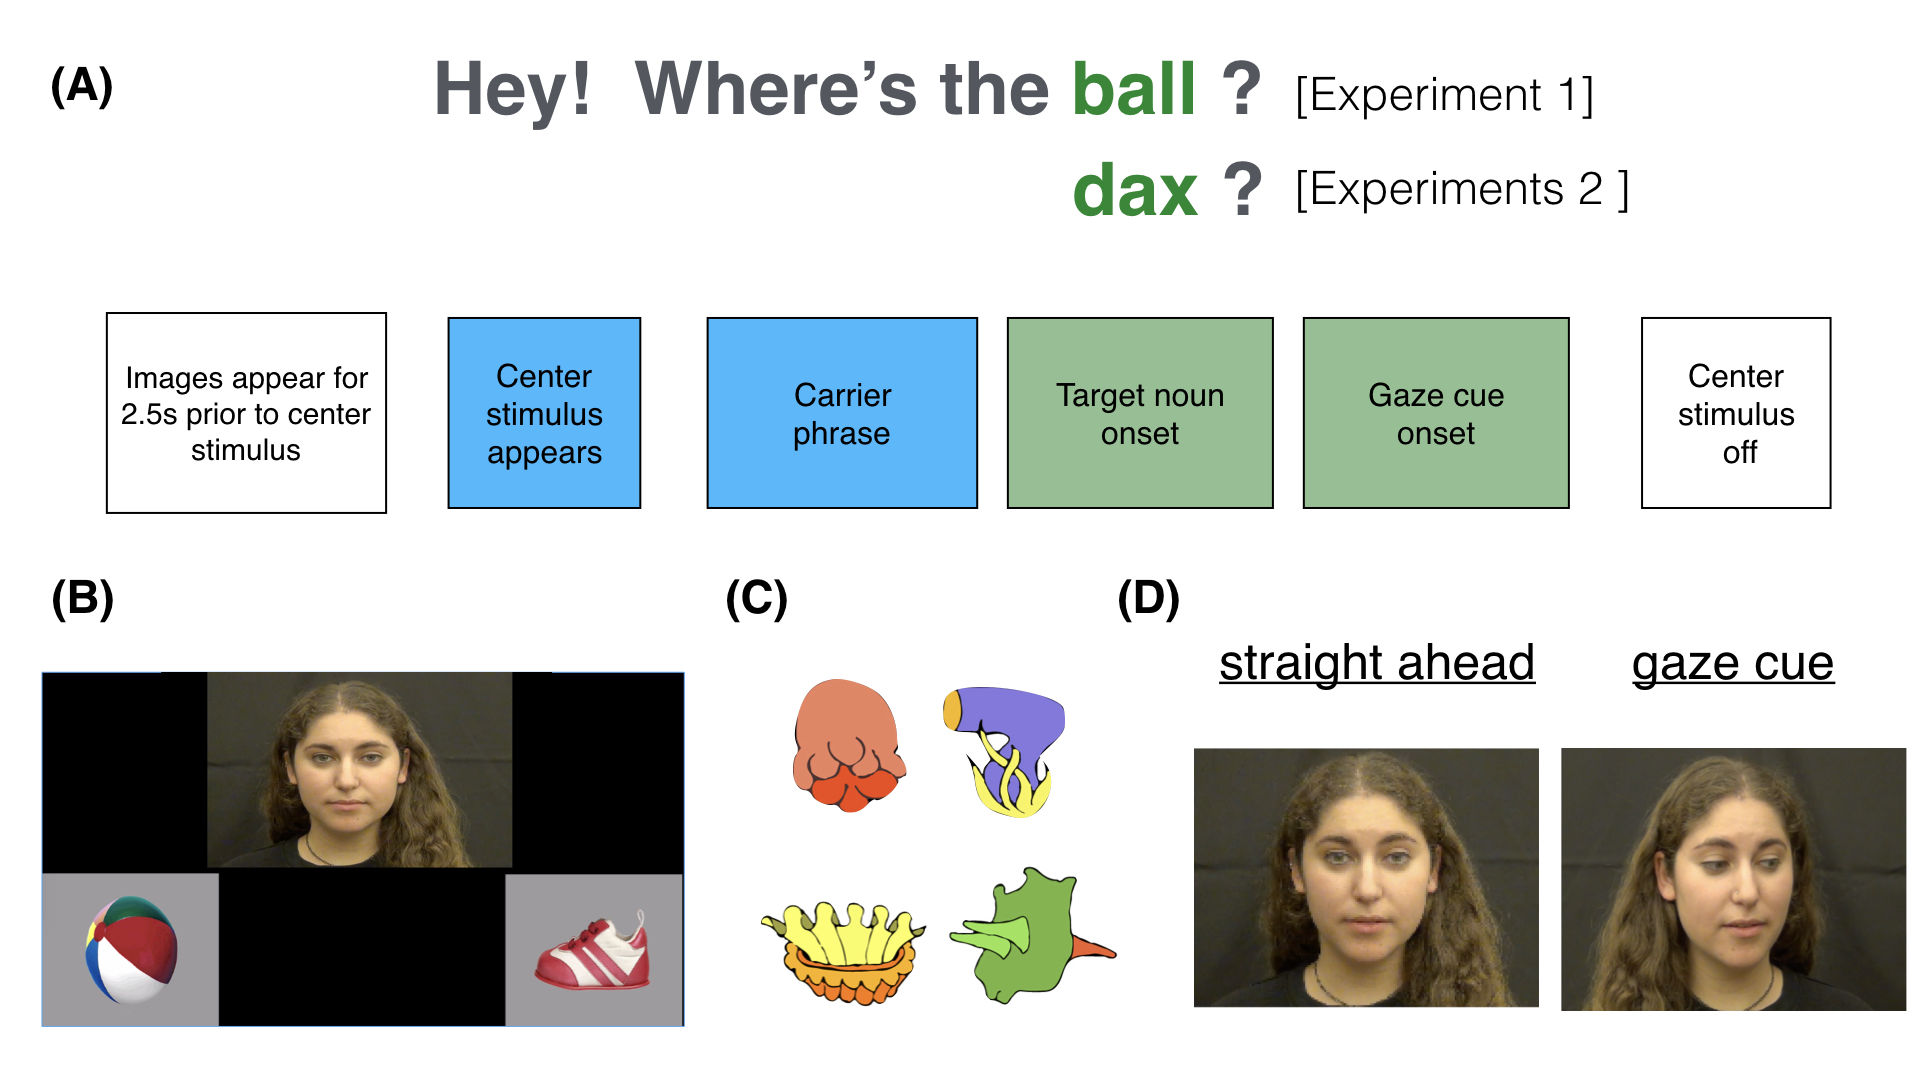
\includegraphics[width=0.9\linewidth]{/Users/kylemacdonald/Documents/Projects/SPEED-ACC-NOVEL/writing/figures/plots/gaze_stimuli} 

}

\caption{Stimuli for Experiments 1, 2, and 3. Panel A shows the structure of the linguistic stimuli for a single trial. Panel B shows the layout of the fixation locations for all tasks: the center stimulus, the target, and the distracter. Panel C shows a sample of the images used as novel objects in Experiment 3. Panel D shows an example of the social gaze manipulation.}\label{fig:gaze-stimuli}
\end{figure}

Participants viewed the task on a screen while their gaze was tracked
using an SMI RED corneal-reflection eye-tracker mounted on an LCD
monitor, sampling at 30 Hz. The eye-tracker was first calibrated for
each participant using a 6-point calibration. On each trial,
participants saw two images of familiar objects on the screen for two
seconds before the center stimulus appeared. Next, they processed the
target sentence -- which consisted of a carrier phrase, a target noun,
and a question -- followed by two seconds without language to allow for
a response. Both children and adults saw 32 trials (16 gaze trials; 16
no-gaze trials) with several filler trials interspersed to maintain
interest. The gaze manipulation was presented in a blocked design with
the order of block counterbalanced across participants.

\subsection{Results and Discussion}\label{results-and-discussion}

\emph{Timecourse looking.} We first analyzed how the presence of gaze
influenced listeners' distribution of attention across the three
fixation locations while processing familiar words. At target-noun
onset, listeners tended to look more at the speaker than the objects. As
the target noun unfolded, the mean proportion looking to the center
decreased as participants shifted their gaze to the images. Proportion
looking to the target increased sooner and reached a higher asymptote
compared to proportion looking to the distracter for both gaze
conditions with adults spending more time looking at the target compared
to children. After looking to the named referent, listeners tended to
shift their gaze back to the speaker's face.

\begin{figure}[!t]

{\centering 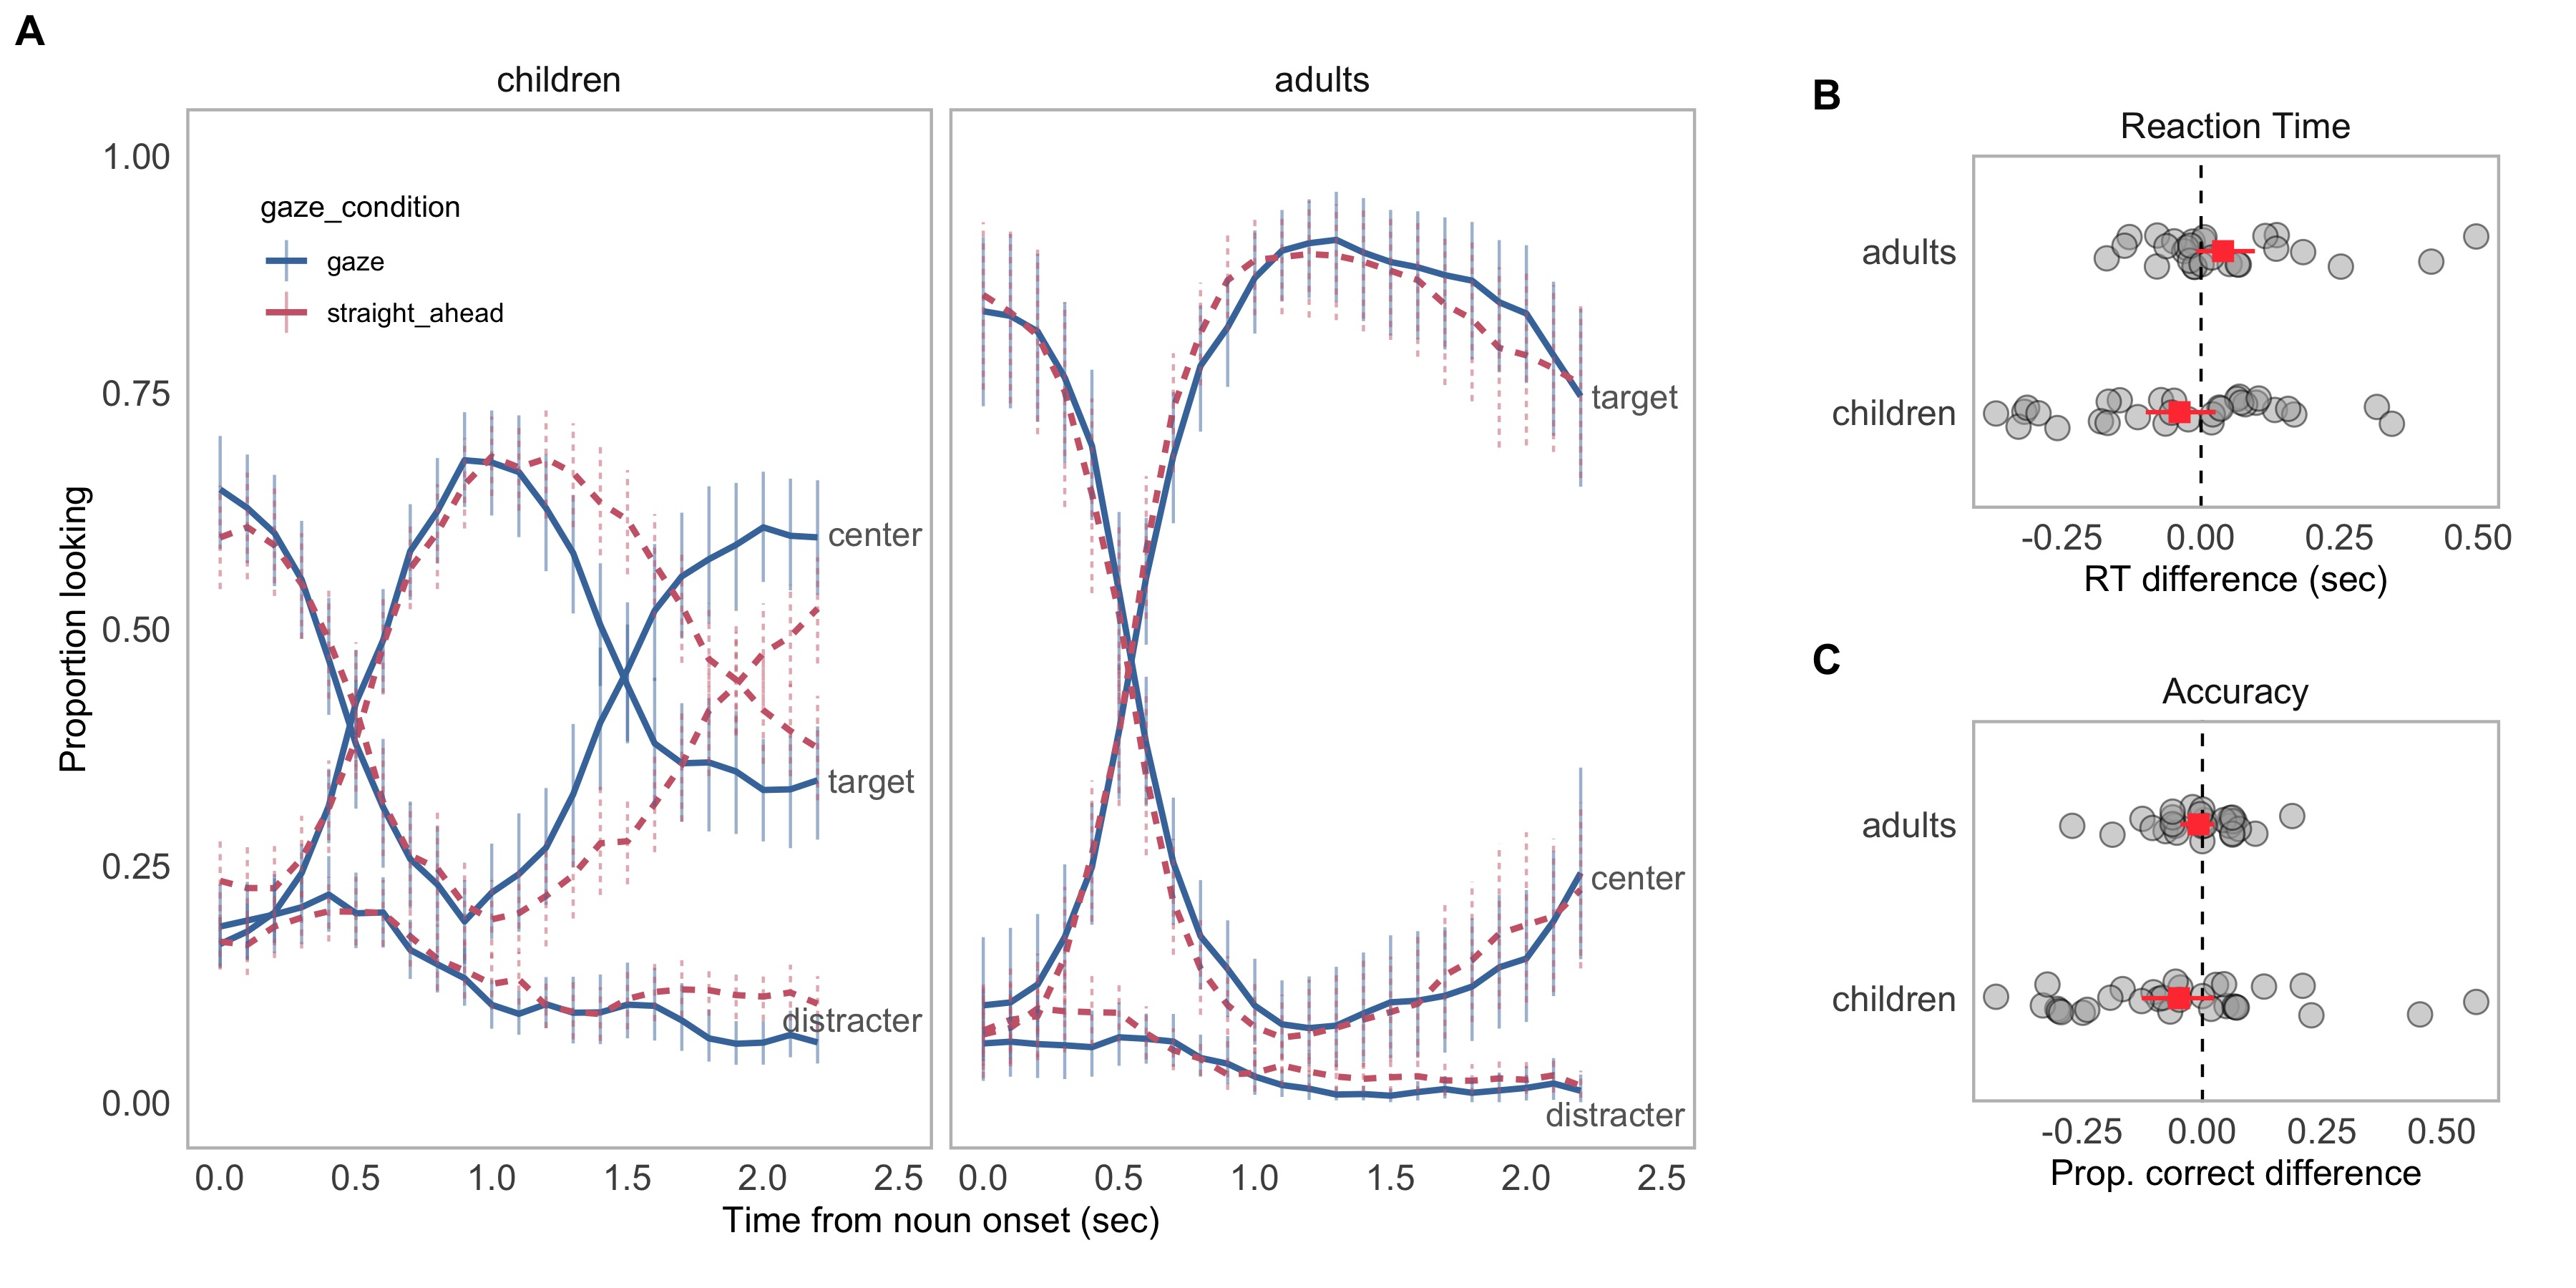
\includegraphics[width=0.95\linewidth]{/Users/kylemacdonald/Documents/Projects/SPEED-ACC-NOVEL/writing/figures/plots/speed_acc_fam_behav} 

}

\caption{Timecourse looking, first shift Reaction Time (RT), and Accuracy results for children and adults in Experiment 1. Panel A shows the overall looking to the center, target, and distracter stimulus for each gaze condition and age group. Panel B shows the distribution of pairwise contrasts between each participant's RT in the gaze and no-gaze conditions. The square point represents the group means. The vertical dashed line represents the null model of zero condition difference. Error bars represent the 95\% HDI. Panel C shows the same information but for first shift accuracy.}\label{fig:speed-acc-gaze-results}
\end{figure}

We did not see evidence that the presence of a post-nominal gaze cue
changed how children or adults allocated attention early in the target
word. Children in the gaze condition, however, tended to shift their
focus back to the speaker earlier after shifting gaze to the named
object and spent more time fixating on the speaker's face throughout the
rest of the trial (\(p < .001\); nonparametric cluster-based permutation
analysis). Next, we ask how these different processing contexts changed
the timing and accuracy of children's initial decisions to shift away
from the center stimulus.

\emph{First shift RT and Accuracy.} To quantify differences across the
groups, we fit a Bayesian linear mixed-effects regression predicting
first shift RT as a function of gaze condition and age group:
\emph{Log(RT) \(\sim\) gaze condition + age group + (gaze\_condition +
item \textbar{} subject)}. Both children and adults generated similar
RTs in the gaze (children \(M_{rt}\) = 563.16 ms, adults \(M_{rt}\) =
652.40 ms) and no-gaze (children \(M_{rt}\) = 575.76 ms, adults
\(M_{rt}\) = 608.31 ms) conditions, with the null value of zero
condition differences falling within the 95\% credible interval
(\(\beta\) = -0.36, 95\% HDI {[}-0.89, 0.06{]}). Next, we fit the same
model to estimate first shift accuracy. Adults generated more accurate
gaze shifts (\(M\) = 0.90) compared to children (\(M\) = 0.64) with the
null value falling outside the 95\% HDI (\(\beta_{age}\) = -1.76, 95\%
HDI {[}-2.19, -1.34{]}). Similar to the RT analysis, we did not find
strong evidence of a difference in performance across the gaze
conditions (\(\beta\) = 0.10, 95\% HDI {[}-0.18, 0.41{]}).

Taken together, the time course and first shift analyses suggest that
hearing a familiar noun was sufficient for both adults and children to
shift visual attention away from the speaker and seek a named referent.
Neither age group showed evidence of delaying their eye movements to
gather a social cue to reference that could have provided additional
disambiguating information. The presence of gaze, however, did change
children's looking behavior such that they were more likely to allocate
attention to the speaker after processing the familiar noun. While we
did not predict these results, it is interesting that listeners did not
delay their eye movements to seek social information when processing
familiar words. This behavior seems reasonable if eye movements during
familiar language processing are highly-practiced visual routines such
that seeking a post-nominal gaze cue becomes less-relevant to
disambiguating and grounding reference. Moreover, if listeners developed
an expectation that their goal was to seek out named objects quickly,
then fixating on the speaker for longer becomes less goal-relevant.

In previous work, we found that both children and adults fixated longer
on a speaker when processing familiar words in the presence of
background noise (MacDonald, Marchman, Fernald, \& Frank, 2018). We
explained this result as listeners adapting to the informational demands
of the environment such that they gathered additional visual information
when it was useful for language comprehension. The results of Experiment
1 can constrain this information seeking explanation by showing that
listeners do not always seek social information when it is available;
instead, children may take their uncertainty into account and only adapt
their information seeking when ambiguity is higher.

This interpretation raises an interesting question: Would children adapt
gaze patterns to gather more social information when they do not know
word meanings? That is, when surrounded by unfamiliar objects, the value
of seeking visual information from a social partner should increase
since this action could provide relevant disambiguating information -- a
point that has long been emphasized by social-pragmatic theories of
language acquisition (P. Bloom, 2002; Clark, 2009; Hollich et al.,
2000). Experiments 2 and 3 explore this case and ask whether learners
would adapt their gaze patterns to seek information from social partners
in the context of processing novel words.

\section{Experiment 2}\label{experiment-2}

Because children process language in environments with multiple possible
referents, learning the meaning of even the simplest word requires
reducing this uncertainty. A cross-situational statistical learner can
aggregate across ambiguous naming events to learn stable word meanings.
But for this aggregation process to work, learners must allocate their
limited attention and memory resources to the relevant statistics in the
world -- how do they select what information to store?

In prior work (MacDonald, Yurovsky, \& Frank, 2017), we found that the
presence of a gaze cue shifted adults away from storing multiple
word-object links and towards tracking a single hypothesis. Those
experiments, however, relied on an offline measurement of word learning
(a button press on test trials) and an indirect measure of attention
during learning (self-paced decisions about how long to inspect the
visual scene during learning trials). We address these limitations in
Experiment 2 by adapting the social cross-situational learning paradigm
to use eye-tracking methods. By moving to an eye-tracking procedure, we
could ask: (1) how does the presence of gaze alter learners'
distribution of visual attention between objects and the speaker? And
(2) does the presence of a gaze cue change the strength of the
relationship between real-time information selection during learning and
long-term retention of word-object links?

\subsection{Methods}\label{methods-1}

\subsubsection{Participants}\label{participants-1}

34 undergraduate students were recruited from the Stanford Psychology
One credit pool (17 F). Four participants were excluded during analysis
because the eye-tracker did not correctly record their gaze coordinates.
The final sample included 30 participants.

\subsubsection{Materials}\label{materials-1}

The experiment featured sixteen pseudo-words recorded by an AT\&T
Natural VoicesTM speech synthesizer using the \enquote{Crystal} voice (a
woman's voice with an American English accent), as well as 48 novel
objects represented by black-and-white drawings of fictional objects
from Kanwisher, Woods, Iacoboni, and Mazziotta (1997). Sixteen words
were used so that the experiment would be sufficiently long to make
within-subject comparisons across trials, and 48 objects were used so
that objects would not be repeated across trials. Six familiar objects
from the same set of drawings were used for the two practice trials,
accompanied by two familiar words using the same speech synthesizer.
Finally, the videos of the speaker's face were taken from MacDonald et
al. (2017).

\subsubsection{Procedure}\label{procedure-1}

We tracked adults' eye movements while they watched a series of
ambiguous word-learning events (16 novel words) organized into pairs of
exposure and test trials (32 trials total). All trials consisted of a
set of two novel objects and one novel word. Participants were randomly
assigned to either the Gaze condition in which a speaker looked at one
of the objects on exposure trials or the No-Gaze condition in which a
speaker looked straight on exposure trials. Every exposure trial was
followed by a test trial, where participants heard the same novel word
paired with a new set of two novel objects. One of the objects in the
set had appeared in the exposure trial (\enquote{target} object), while
the other object had not previously appeared in the experiment
(\enquote{distracter} object).

\begin{figure}[!t]

{\centering 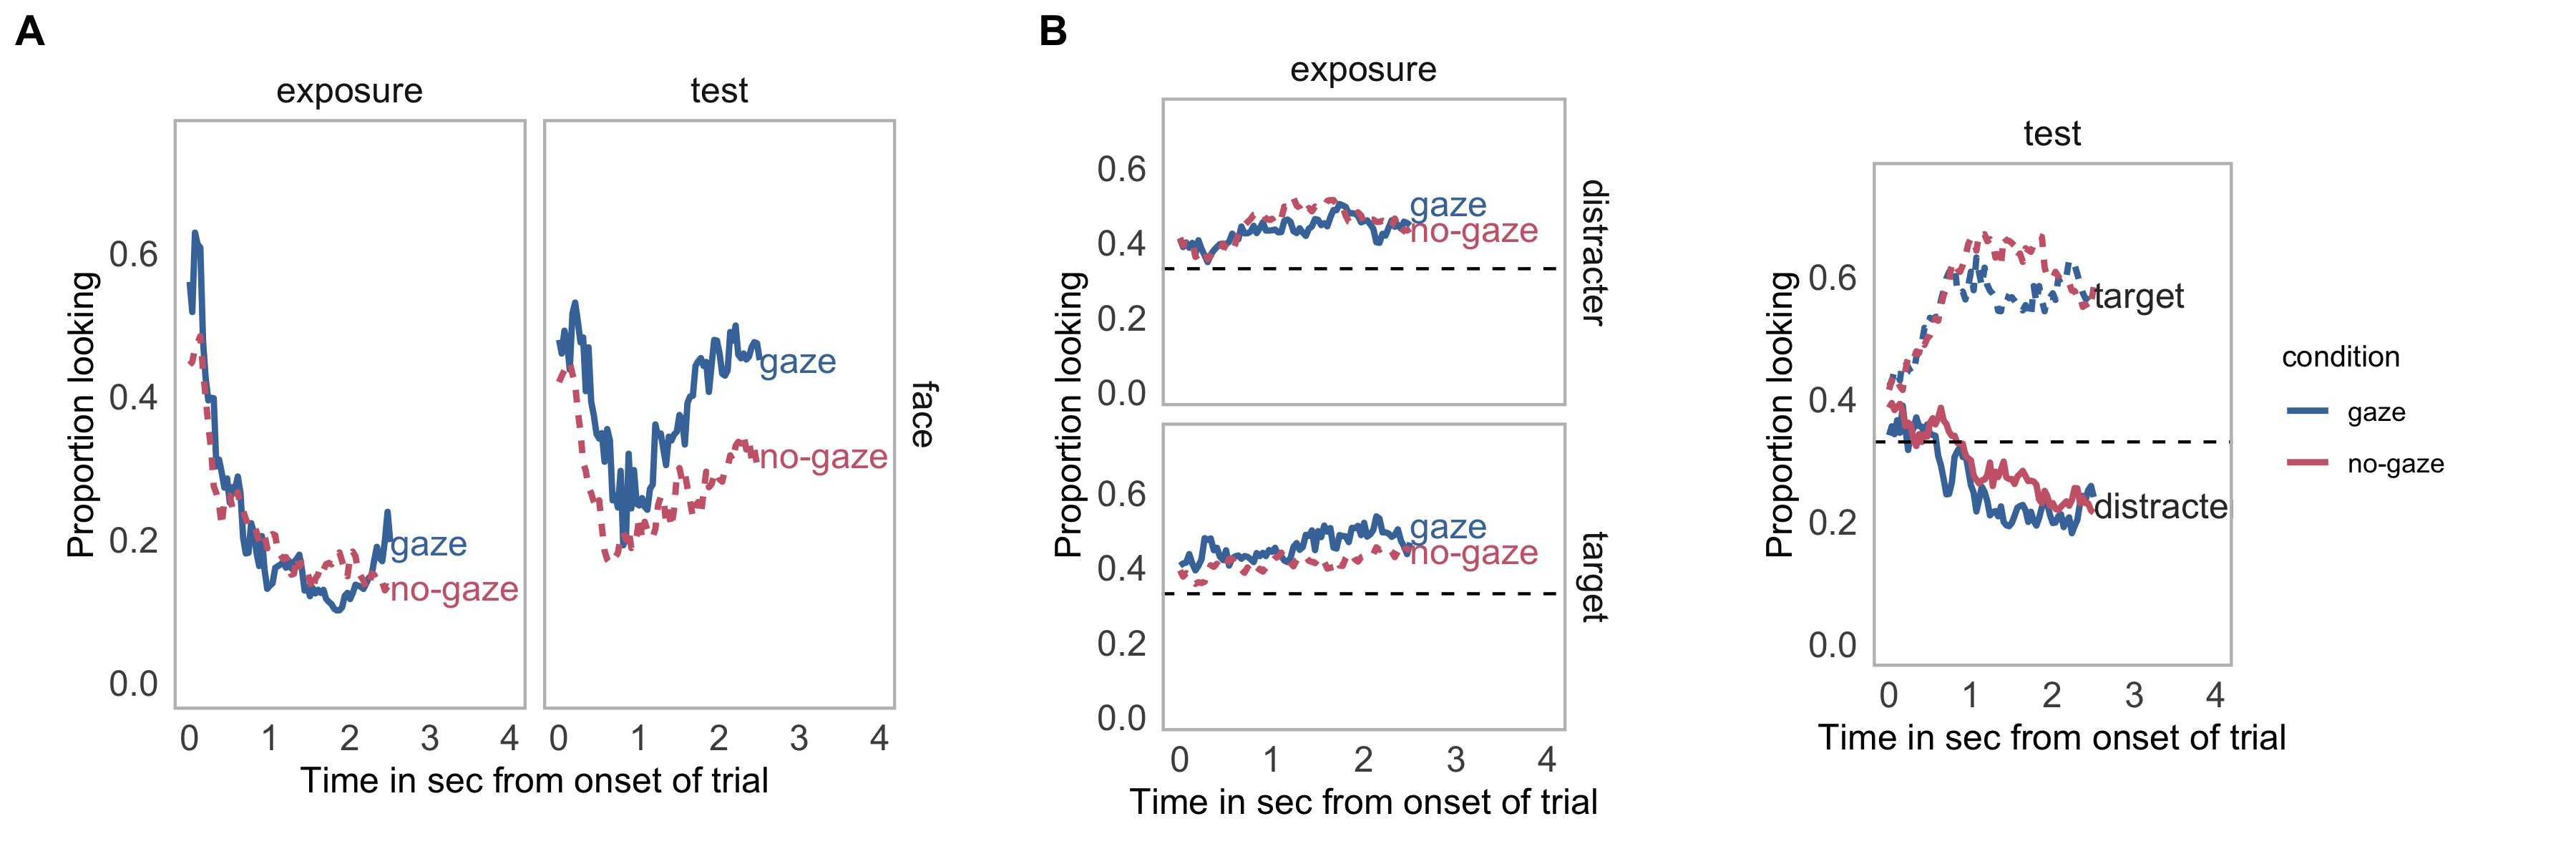
\includegraphics[width=1\linewidth]{/Users/kylemacdonald/Documents/Projects/SPEED-ACC-NOVEL/writing/figures/plots/gaze_xsit_tc} 

}

\caption{Overview of adults' looking to the three fixation targets (Face, Target, Distracter) over the course of the trial. Panel A shows proportion looking to the speaker's face for exposure and test trials. Color and line type represent gaze condition. Panel B shows the same information but for proportion looking to the target and distracter images.}\label{fig:gaze-xsit-tc-plot}
\end{figure}

The side of the screen of the target object was counterbalanced
throughout the experiment. In the gaze condition, for half of the test
trials, the target object was the focus of the speaker's gaze during the
exposure trial, while the other half, the target object was the object
that had not been the focus of gaze during labeling.

\subsection{Results and Discussion}\label{results-and-discussion-1}

\emph{Timecourse looking.} The first question of interest was how did
the presence of a gaze cue change adults' distribution of attention
across the three fixation locations while processing language in
real-time? Figure~\ref{fig:gaze-xsit-tc-plot} presents an overview of
looking to each AOI for each processing context. At the target-noun
onset, adults tended to look more at the speaker's face on both exposure
and test trials. As the target noun unfolded, the mean proportion
looking to the center decreased as participants shifted their gaze to
the target or the distracter images. On exposure trials, adults tended
to distribute their attention relatively evenly across target and
distracter images. On test trials, proportion looking to the target
increased sooner and reached a higher asymptote compared to proportion
looking to the distracter for both conditions, suggesting that adults
were able to track the consistent word-object links both with and
without accompanying social information.

There were several qualitative differences in looking behavior across
the different gaze conditions and trial types. First, adults spent more
time looking to a speaker's face when she provided a social gaze cue,
especially on test trials that were preceded by gaze (Figure
~\ref{fig:gaze-xsit-tc-plot}A). Second, adults in the gaze condition
looked slightly more to the target image throughout the trial. This
behavior is reasonable since half of the trials, the speaker's gaze was
focused on the target image that would appear on the subsequent test
trial. Third, on test trials, adults looked more to the images in the
no-gaze condition, which led to a higher proportion of looking to the
target and a higher proportion of looking to the distracter images
(Figure ~\ref{fig:gaze-xsit-tc-plot}B).

\begin{figure}[!t]

{\centering 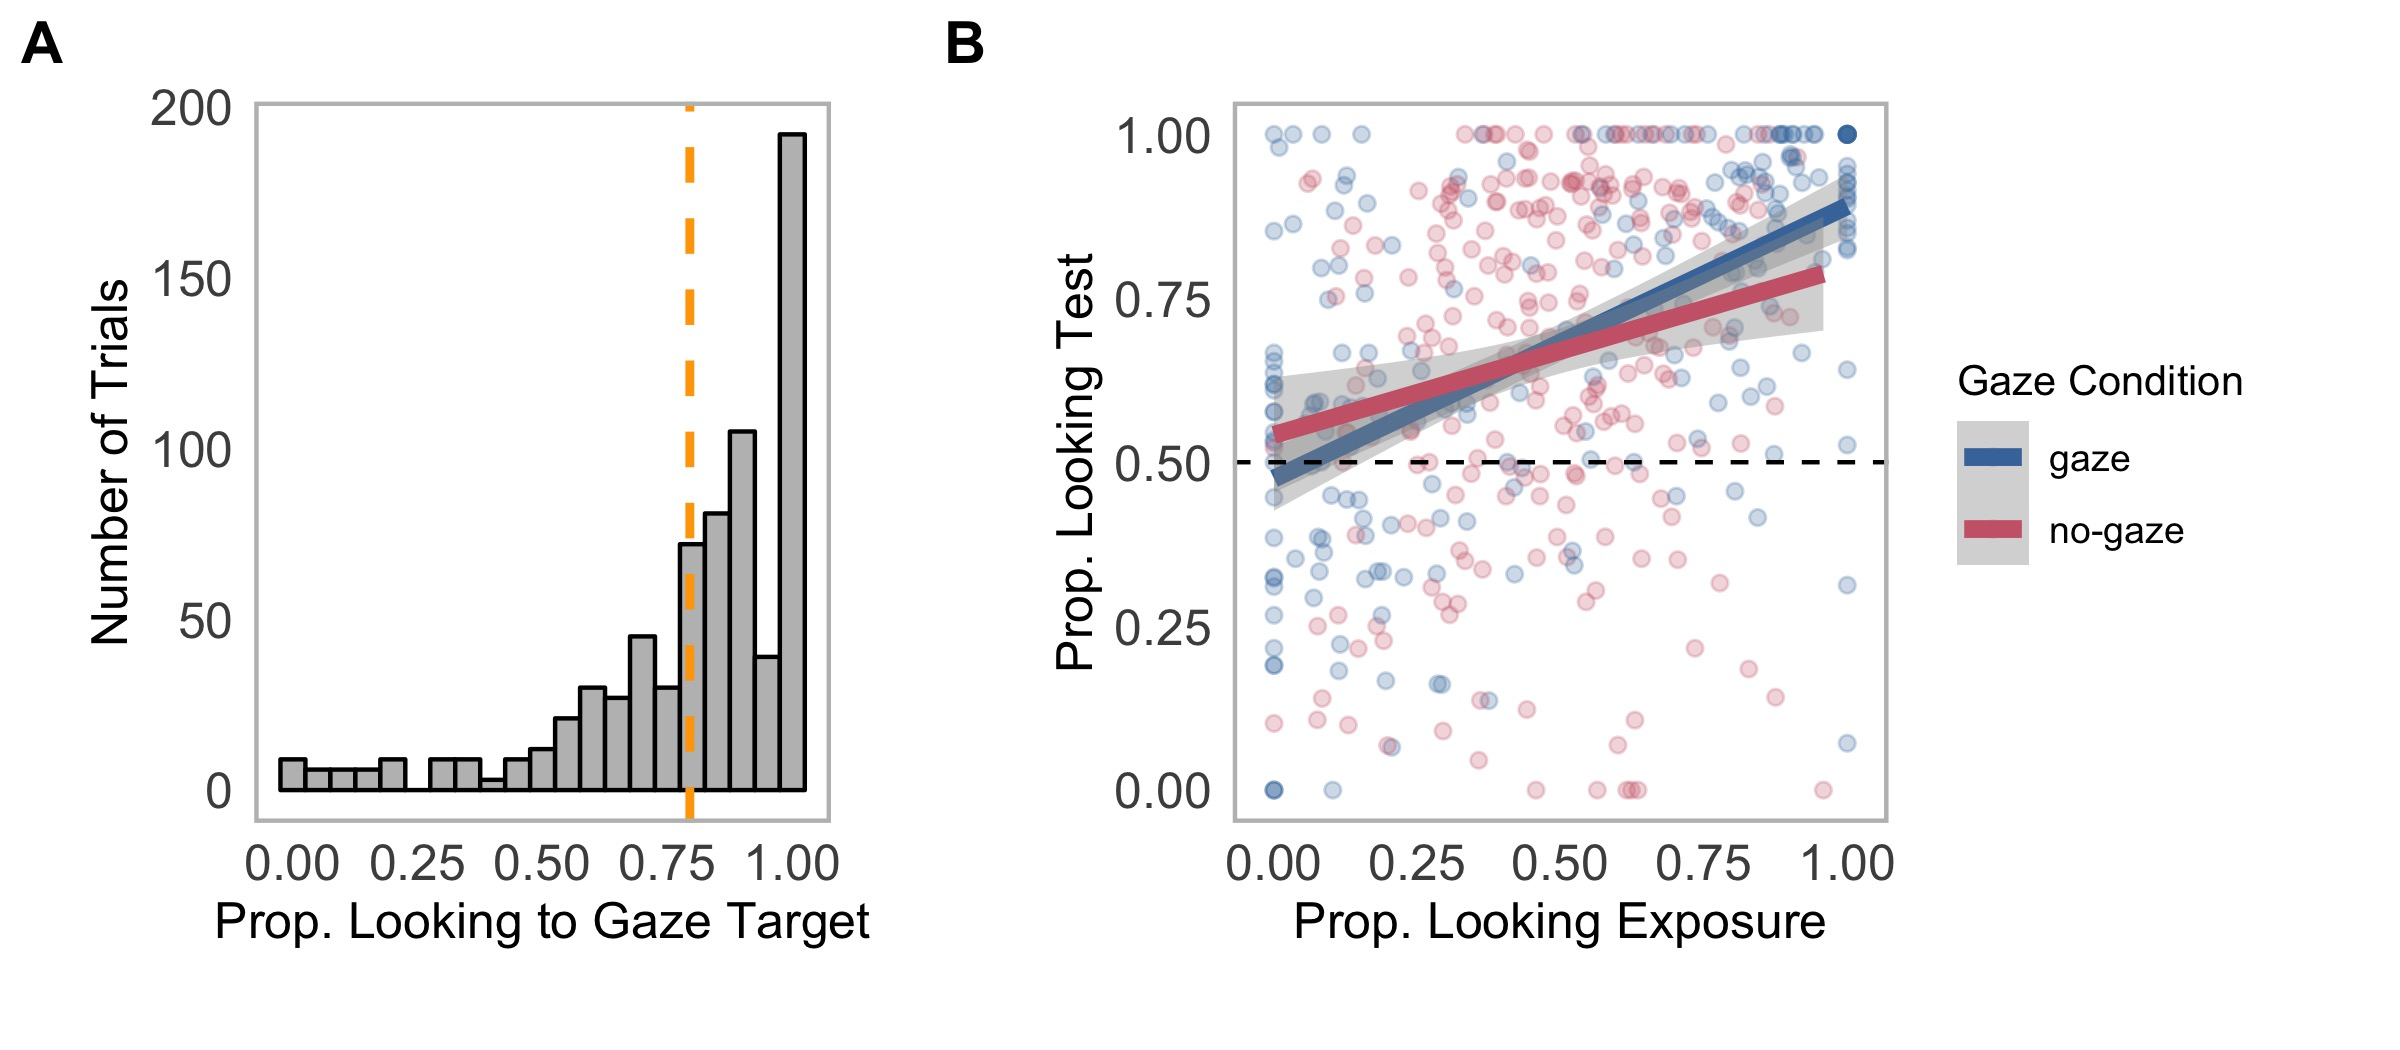
\includegraphics[width=0.9\linewidth]{/Users/kylemacdonald/Documents/Projects/SPEED-ACC-NOVEL/writing/figures/plots/gaze_xsit_prop_looking} 

}

\caption{Panel A shows participants’ tendency to look at the object that was the target of the speaker’s gaze on exposure trials. The vertical, dashed line represents the mean proportion of time looking to the gaze target across all trials. Panel B shows the relationship between adults' looking behavior on exposure and test trials for the gaze and no-gaze conditions. The lines represent linear model fits.}\label{fig:gaze-xsit-prop-looking-plot}
\end{figure}

\emph{Relationship between performance on exposure and test trials.}
When the speaker generated a social cue during labeling, adults reliably
followed that cue and tended to focus their attention on a single object
(Figure ~\ref{fig:gaze-xsit-prop-looking-plot}A). In contrast, people in
the No-gaze condition tended to distribute their attention more broadly
across the two objects. For adults in both gaze contexts, more time
spent attending to the target object on exposure trials led higher
proportion looking to the target, i.e., better recall, at test
(\(\beta_{exposure}\) = 0.43, 95\% HDI {[}0.36, 0.50{]}). Critically,
there was an interaction between the gaze condition and the effect of
exposure looking patterns (Figure
~\ref{fig:gaze-xsit-prop-looking-plot}B): When a speaker's gaze guided
adults' visual attention, they showed stronger memory for the
newly-learned word-object link (\(\beta_{int}\) = -0.19, 95\% HDI
{[}-0.33, -0.04{]}).

Together, the time course and proportion looking results suggest that
the presence of gaze led adults to spend more time fixating on the
speaker, which, in turn, changed how they distributed fixations across
the target and distracter objects during labeling events. Moreover, when
learners followed the gaze cue, they showed a stronger relationship
between visual attention on exposure trials and target looking on test
trials, suggesting that seeking social information modulated the
fidelity with which learners' stored potential word-object links.

\subsubsection{Limitations}\label{limitations}

There were several limitations to this study. First, the linguistic
stimulus occurred at the trial onset when the images and the speaker
appeared on the screen. This trial structure makes it challenging to
interpret learners' initial decisions to stop gathering information from
a social target to fixate the objects, a behavior that we have used in
our prior work to shed light on how children's information selection
adapts to their processing environment (MacDonald et al., 2018). Second,
the linguistic stimuli consisted of pseudowords recorded by a speech
synthesizer and presented in isolation, thus removing any sentential
context. Presenting isolated words is unlikely to work with the target
age range for this research. Finally, we used a minimal
cross-situational learning paradigm with only two exposures to each
word-object link, which does not allow for measurement of the effect of
accumulating statistical information over a longer timescale. Thus,
Experiment 3 was designed to address these limitations, allowing us to
ask how younger learners' information seeking from social partners
changes as a function of increased exposure to consistent word-object
mappings.

\section{Experiment 3}\label{experiment-3}

Experiment 3 explores whether learners' real-time information seeking
from social partners adapts as they accumulate knowledge of word-object
links.\footnote{See \url{https://osf.io/nfz85/} for a pre-registration
  of the analysis plan and predictions.} We also set out to address the
limitations of Experiment 2 by making two key modifications to the
social, cross-situational learning paradigm. First, we included more
than two exposures to a novel word-object link, allowing us to measure
changes in learners' integration of social and statistical information
over a longer timescale. Second, we changed the linguistic stimuli to
use the trial structure in Experiment 1 such that the novel words
occurred within a sentence spoken in a child-friendly register. This
change allowed us to analyze children's first gaze shifts away from a
social target and ask how the threshold of information gathering changed
as a function of statistical learning about word-object mappings.

We aimed to answer the following specific research questions:

\begin{enumerate}
\def\labelenumi{\arabic{enumi}.}
\tightlist
\item
  Does the presence of gaze change whether listeners seek social
  information?\\
\item
  Does social information seeking (looks to speakers vs.~objects) change
  as a function of repeated exposures to a word-object link?
\item
  Does following a gaze cue change the relationship between visual
  attention during labeling and memory of word-object links?
\end{enumerate}

To answer these questions, we compared the timing and accuracy of eye
movements during a real-time cross-situational word learning task where
participants processed sentences containing a novel word (e.g.,
\enquote{Where's the \emph{dax}?}) while looking at a simplified visual
world with three fixation targets (a video of a speaker and two images
of unfamiliar objects).

\subsection{Predictions}\label{predictions}

We had three key behavioral predictions. First, the presence of a gaze
cue will change participants' decisions about visual fixation. We
hypothesize that a post-nominal gaze cue increases the value of fixating
on a speaker. This manipulation will cause participants to allocate more
fixations to the speaker when gaze is present, leading to slower first
shift reaction times and higher proportion looking, especially earlier
in learning (i.e., lower trial numbers within each block of exposure
trials to a novel word-object pairing). We operationalize this
prediction as a main effect of Gaze condition on RT, and a trial number
by Gaze condition interaction such that the decrease in RT will be
greater on exposure trials in the Gaze condition.

Second, participants' distribution of attention to speakers compared to
objects will shift throughout learning. Early in the task, participants
will allocate more fixations to a speaker to prioritize gathering visual
information that disambiguates reference. After experiencing multiple
exposures to a word-object pairing, participants will generate faster
gaze shifts, showing signatures of familiar language comprehension. We
further predict that later in learning blocks, participants will
allocate more fixations to the objects, displaying looking patterns that
could support learning long-term associations between words and objects.

Third, the presence of gaze should lead to a stronger link between words
and objects, resulting in faster learning, which we operationalize as
more accurate first shifts, faster RTs, and a higher proportion looking
to the target object in the gaze condition.

\subsection{Methods}\label{methods-2}

\subsubsection{Participants}\label{participants-2}

Participants were native, monolingual English-learning children (\(n=\)
NA; NA F) and adults (\(n=\) 30; 20 F). All participants had no reported
history of developmental or language delay and normal vision. 6 adults
were run but not included in the analysis because they were not native
speakers of English. 7 children participants were run but not included
in the analysis because the participant did not complete more than half
of the trials in the task.

\subsubsection{Materials}\label{materials-2}

\emph{Linguistic stimuli.} The video/audio stimuli were recorded in a
sound-proof room and featured two female speakers who used natural
child-directed speech and said one of two phrases: \enquote{Hey! Can you
find the (novel word)} or ``Look! Where's the (novel word). The target
words were four pseudo-words: bosa, modi, toma, and pifo. The novel
words varied in length (shortest = 472.00 ms, longest = 736.00 ms) with
an average length of 606.31 ms.

\emph{Gaze manipulation}. To create the stimuli in the gaze condition,
the speaker waited until she finished producing the novel word before
turning her head to gaze at the bottom right corner of the frame. After
looking at the named object, she then returned her gaze to the center of
the frame. We chose to allow the length of the gaze cue to vary to keep
the stimuli naturalistic. The average length of gaze was 2.06 seconds
with a range from 1.74 to 2.67 seconds.

\emph{Visual stimuli.} The image set consisted of 28 colorful digitized
pictures of objects that were selected such that they would be
interesting to and that children would be unlikely to have already a
label associated with the objects. The side of the target picture was
counterbalanced across trials.

\subsubsection{Procedure}\label{procedure-2}

Participants viewed the task on a screen while their gaze was tracked
using an SMI RED corneal-reflection eye-tracker mounted on an LCD
monitor, sampling at 30 Hz. The eye-tracker was first calibrated for
each participant using a 6-point calibration. Then, participants watched
a series of ambiguous word learning events organized into pairs of one
exposure and one test trial. On each trial, participants saw of a set of
two unfamiliar objects and heard one novel word.

Each word was learned in a block of four exposure-test pairs for a total
of eight trials for each novel word. Critically, on each trial within a
word block, one of the objects in the set had appeared on the previous
trials (target object), while the other object was a randomly generated
novel object not previously shown in the experiment (distracter object).
Both children and adults saw 32 trials (16 gaze trials; 16 no-gaze
trials) with several filler trials interspersed to maintain interest.
The gaze manipulation was presented in a blocked design with the order
of block counterbalanced across participants.

\subsection{Results and Discussion}\label{results-and-discussion-2}

\subsubsection{Timecourse looking}\label{timecourse-looking}

\begin{figure}[!t]

{\centering 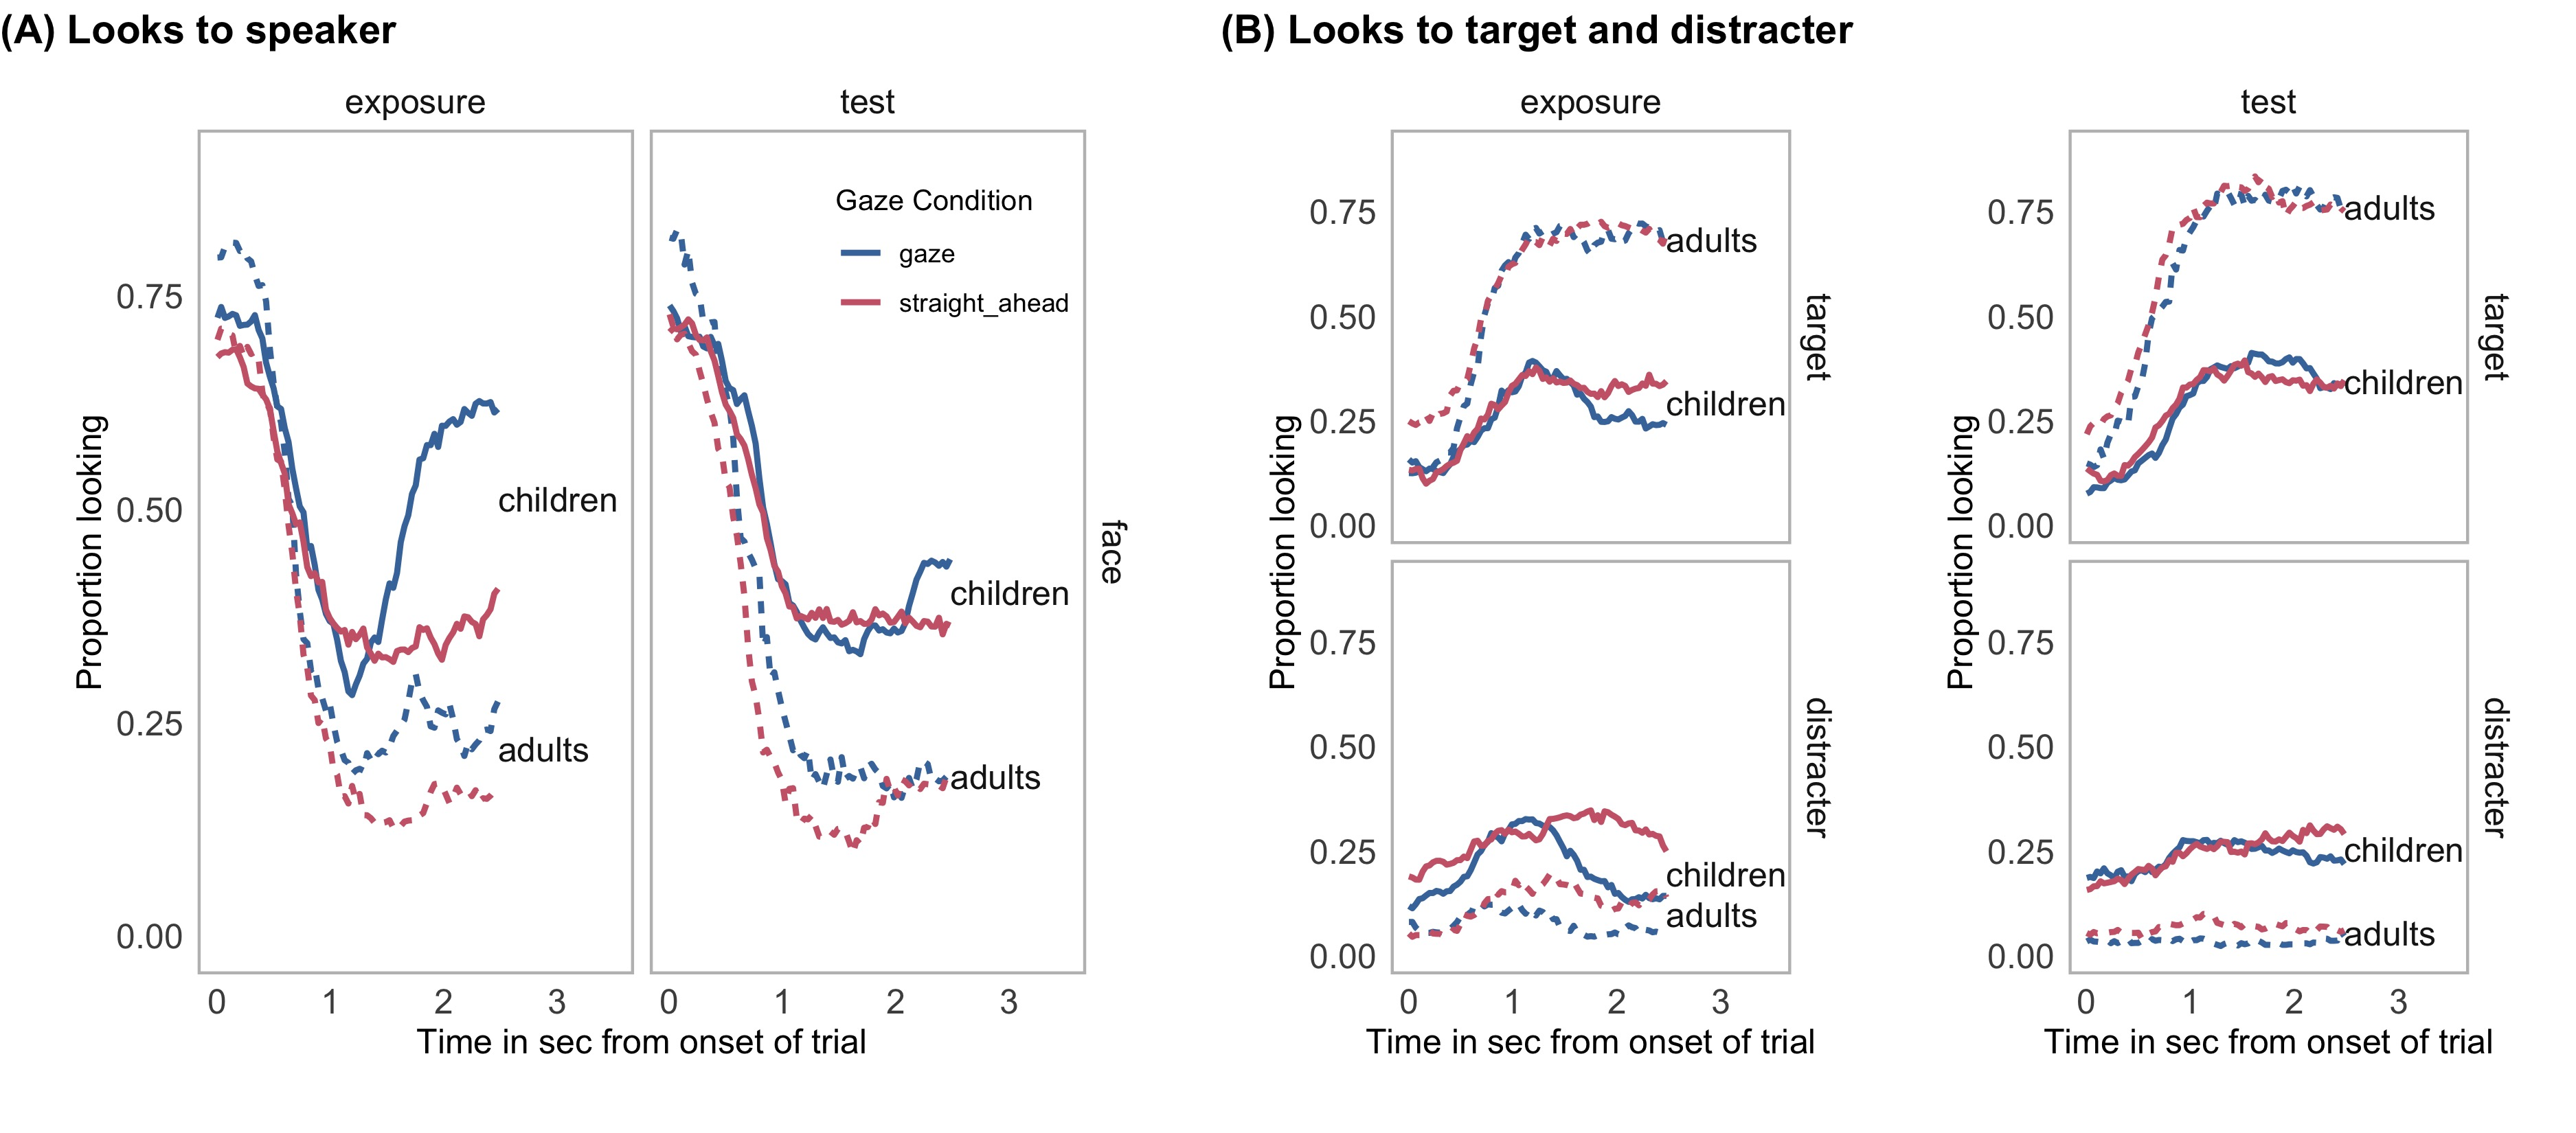
\includegraphics[width=1\linewidth]{/Users/kylemacdonald/Documents/Projects/SPEED-ACC-NOVEL/writing/figures/plots/speed_acc_novel_tc} 

}

\caption{Overview of children and adults' looking to the three fixation targets (Speaker, Target, Distracter) over the course of exposure and test trials. Panel A shows proportion looking to the speaker's face with color indicating gaze condition and line type indicating age group. Panel B shows the same information but for proportion looking to the target and distracter images.}\label{fig:san-tc-plot}
\end{figure}

\emph{Looking to the speaker.} How did the presence of a gaze cue change
learners' decisions to fixate on the speaker? Visual inspection of
Figure ~\ref{fig:san-tc-plot}A shows that both children and adults
tended to start looking at the speaker at noun onset and shifted their
gaze away as the noun unfolded, with adults doing so sooner compared to
children. On Exposure trials when there was a gaze cue, both adults and
children tended to look more to the face at noun onset as indicated by
the higher intercept of the blue curves. Moreover, around one second
after noun onset, listeners tended to shift their attention back to the
speaker's face more often and especially so for children. On Test trials
that were preceded by an Exposure trial with a gaze cue, children and
adults tended to look more to the speaker even though there was no gaze
cue present. This pattern suggests that the presence of gaze modulated
learners' expectations of being able to gather disambiguating
information from the speaker on Test trials.

\emph{Looking to the target and distracter.} Next, we asked how learners
divided attention between the target and distracter objects. On Exposure
trials, looking to both objects increased throughout the trial but more
so for looks to the named object as indicated by the higher asymptote of
the target looking curves. Adults spent more time looking to the target
and less time looking to the distracter as compared to children. The
most substantial effect of gaze on the time course of looking was a
tendency for learners to allocate fewer fixations to the distracter
object when there was a gaze cue present.

\subsubsection{Proportion looking}\label{proportion-looking}

\emph{Learning effects.} Both children (\(M_{gaze}\) = 0.57,
\(M_{no-gaze}\) = 0.55) and adults (\(M_{gaze}\) = 0.91, \(M_{no-gaze}\)
= 0.89) showed evidence of learning the novel word-object links, with
the null value of 0.5 falling below the lower bound of the lowest
credible interval for children's target looking in the No-gaze context
(95\% HDI {[}0.51, 0.60{]}). Our primary question of interest was how
exposure to multiple co-occurrences of word-object pairs would change
learners' distribution of attention between the speaker and objects.
Figure ~\ref{fig:san-prop-looking-plot}) shows proportion looking to the
speaker (~\ref{fig:san-prop-looking-plot}A) and the target and
distracter objects (~\ref{fig:san-prop-looking-plot}B) as a function of
trial number within a word learning block. Both children and adults were
more likely to fixate on the speaker when she provided a gaze cue
(\(\beta_{gaze}\) = 0.09, 95\% HDI {[}0.16, 0.01{]}). Moreover, there
was a developmental difference such that children, but not adults, were
more likely to increase their fixations to the speaker over the course
of the learning block (\(\beta_{age:tr.num}\) = -0.07, 95\% HDI
{[}-0.11, -0.04{]}).

\begin{figure}[!t]

{\centering 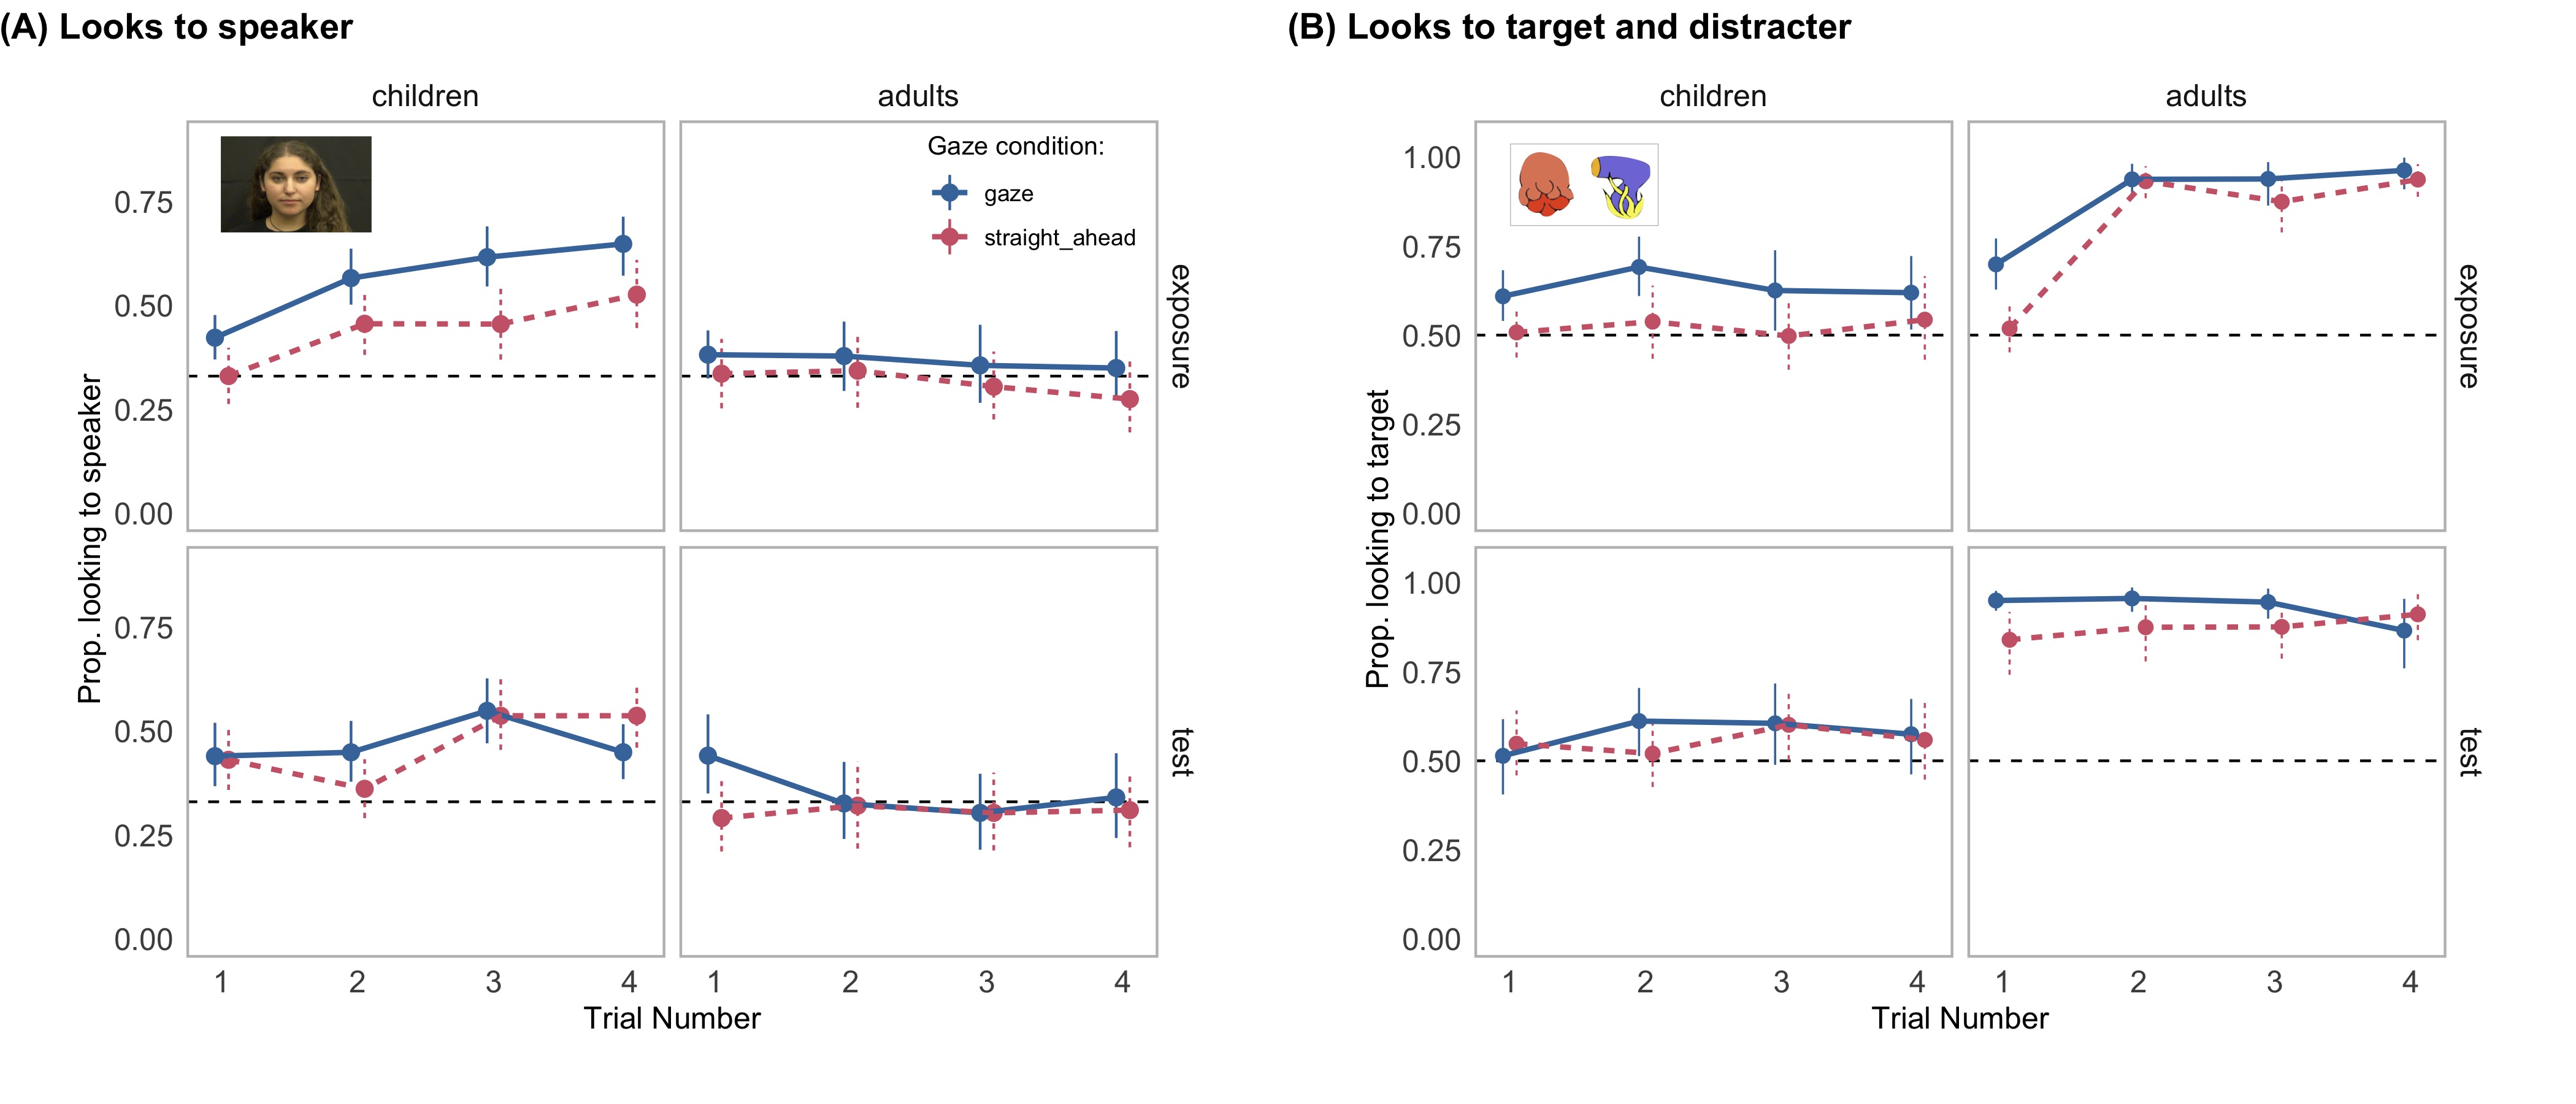
\includegraphics[width=1\linewidth]{/Users/kylemacdonald/Documents/Projects/SPEED-ACC-NOVEL/writing/figures/plots/speed_acc_novel_proplook} 

}

\caption{Panel A shows participants’ tendency to look at the speaker on exposure and test trials as a function of the trial number within a learning block. The horizontal, dashed line represents the tendency to distribute attention equally across the three AOIs. Color indicates gaze condition and error bars represent 95\% credible intervals. Panel B shows the same information but for target and distracter looking across the learning block (left) and aggregated over all trials (right).}\label{fig:san-prop-looking-plot}
\end{figure}

Overall, looking to the target increased as learners were exposed to
more word-object pairings (\(\beta_{tr.num}\) = 0.16, 95\% HDI {[}0.09,
0.24{]}) and was higher when the novel word was accompanied by a gaze
cue (\(\beta_{gaze}\) = 0.14, 95\% HDI {[}0.21, 0.06{]}). Visual
inspection of Figure ~\ref{fig:san-prop-looking-plot} shows that on the
first Exposure trial, both adults and children used the gaze cue to
disambiguate reference, fixating more on the target in the Gaze
condition. For children, higher target looking on Exposure trials with
gaze remained relatively constant across the learning block. In
contrast, adults target looking reached ceiling for both Gaze and
No-gaze conditions by trial number two, indicating that they had
successfully used the co-occurrence information across trials to map the
novel word to its referent. We found an interaction between gaze
condition and trial number such that looking to the target increased
more quickly in the No-gaze condition (\(\beta_{gaze:tr.num}\) = 0.02,
95\% HDI {[}0.00, 0.04{]}), which reflects (1) the higher intercept of
target looking in the presence of gaze and (2) rapid learning of the
word-object association via cross-situational information. Finally,
visual inspection of the proportion looking plot suggests that adults
tended to look more the target when learning from a gaze cue, only
reaching similar levels of accuracy in the no-gaze condition at the end
of the learning block. There was not strong evidence for an effect of
the gaze manipulation on children's looking behavior on Test trials.

\emph{Relationship between looking on exposure and test.} For both
children and adults, more time attending to the target object on
exposure trials led to a higher proportion of looking to the target on
test trials, especially for adults (\(\beta_{exposure:age}\) = 0.16,
95\% HDI {[}0.05, 0.28{]}) and as the number of word-object exposures
increased over the course a learning block (\(\beta_{exposure:tr.num}\)
= 0.07, 95\% HDI {[}0.02, 0.12{]}). There was evidence that participants
in the No-gaze condition showed less learning over the course of each
word block (\(\beta_{gaze:tr.num}\) = -0.02, 95\% HDI {[}-0.04,
0.00{]}). This result dovetails with the findings from Experiment 2,
providing evidence that the presence of social information did more than
change attention on Exposure trials but instead modulated the
relationship between attention during learning and later memory for
word-object links.

Together, the time course and the proportion looking analyses suggest
that the presence of gaze changed how children and adults allocated
attention while processing novel words. In the context of unfamiliar
objects, children tended to fixate more on a speaker's face when she
provided a post-nominal social cue to reference, a difference in looking
behavior that increased as they were exposed to more word-object
co-occurrences. This result is different from the parallel looking
behavior that we found in Experiment 1 where listeners processed highly
familiar nouns. Moreover, in the presence of a speaker who provided a
gaze cue, children and adults spent less time fixating on the distracter
image, which modulates the word-object connections that learners could
store from labeling event. These changes in gaze patterns, however, did
not generalize to performance differences on Test trials for children.
Finally, as in Experiment 2, we found that the presence of a social cue
increased the strength of the link between attention on exposure and
fixations at test.

\subsubsection{First shift RT and
Accuracy}\label{first-shift-rt-and-accuracy}

\begin{figure}[!t]

{\centering 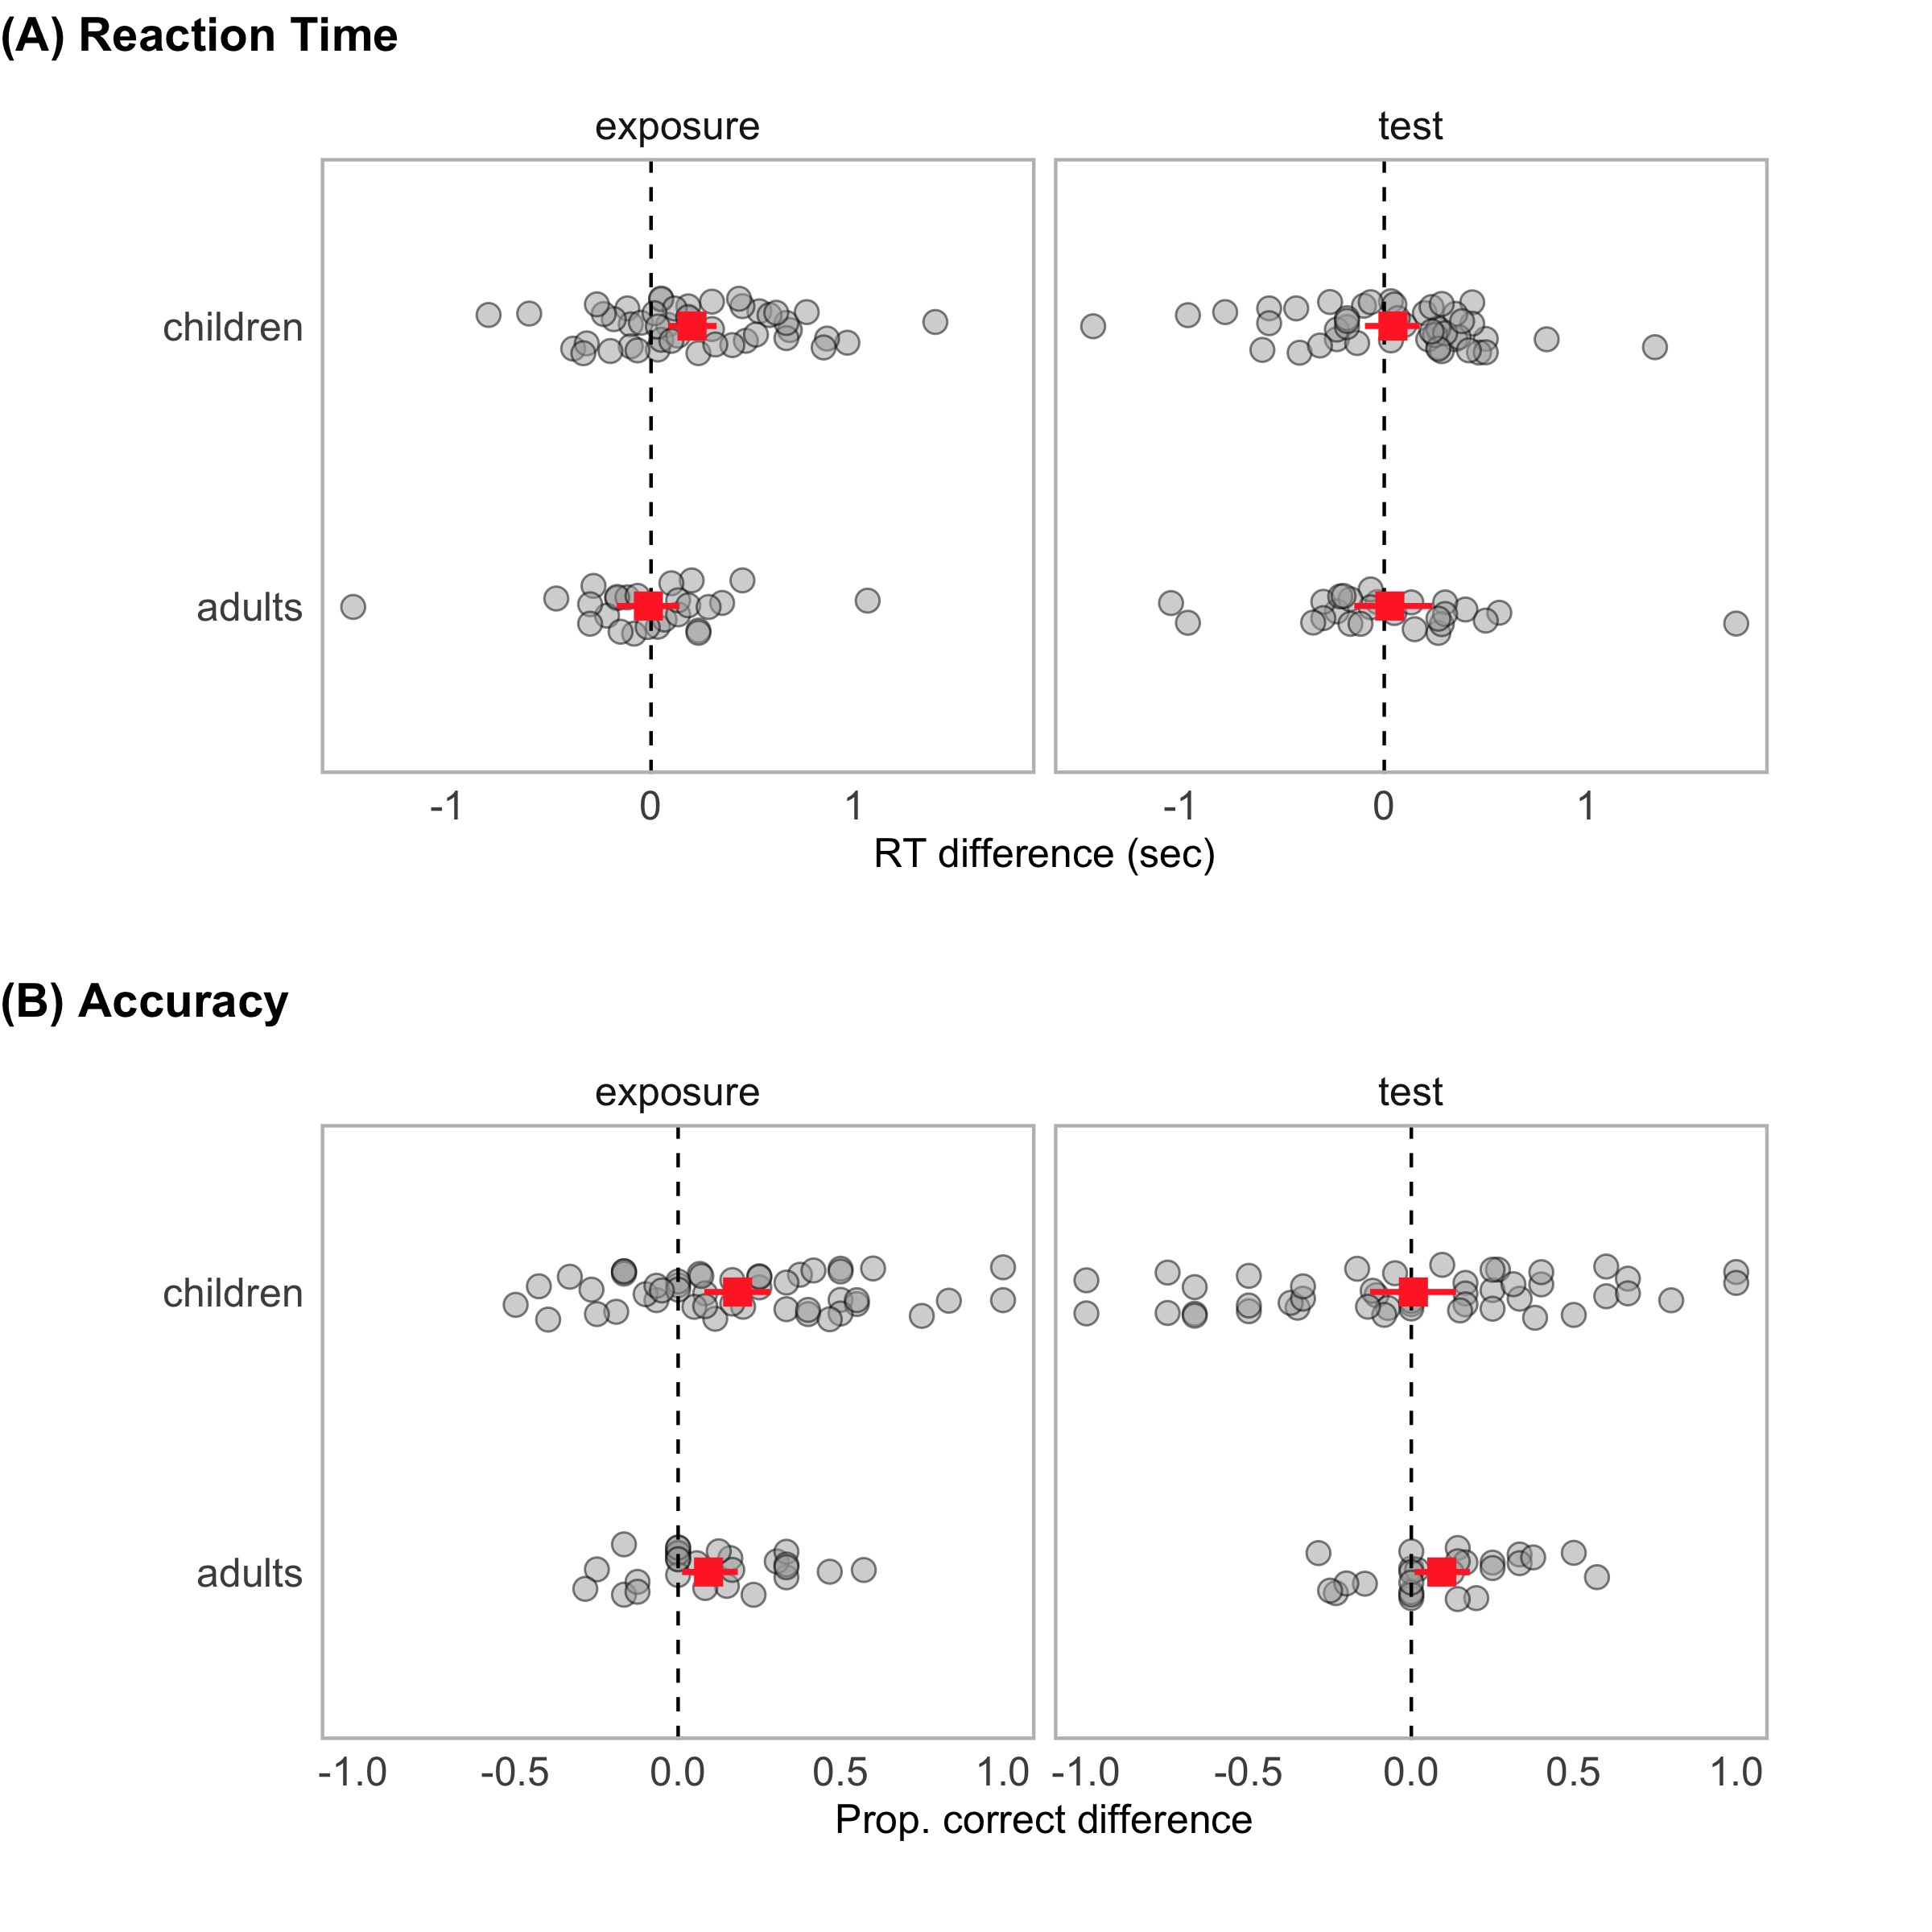
\includegraphics[width=0.8\linewidth]{/Users/kylemacdonald/Documents/Projects/SPEED-ACC-NOVEL/writing/figures/plots/speed_acc_novel_fstshifts} 

}

\caption{First shift Reaction Time (RT), and Accuracy results for children and adults in Experiment 3. Panel A shows the distribution of pairwise contrasts between RTs in the gaze and no-gaze conditions. The square point represents the mean value for each measure. The vertical dashed line represents the null model of zero condition difference. The width each point represents the 95\% HDI. Panel B shows the same information but for participants' first shift accuracy.}\label{fig:speed-acc-novel-shifts}
\end{figure}

We next asked how the presence of gaze influenced learners' decision to
stop gathering visual information from the speaker and start fixating on
the novel objects. To quantify the effect the gaze, we fit a Bayesian
linear mixed-effects regression predicting first shift RT as a function
of whether there was a gaze cue present on the trial and age group. Both
children (Gaze \(M_{rt}\) = 922.41 ms, No-gaze \(M_{rt}\) = 705.22 ms)
and adults (Gaze \(M_{rt}\) = NA ms, No-gaze \(M_{rt}\) = NA ms) fixated
longer on the speaker when she provided a gaze cue (\(\beta_{gaze}\) =
-0.20, 95\% HDI {[}-0.38, -0.01{]}). With no evidence of an interaction
between gaze condition and age group (\(\beta_{age:gaze}\) = 0.27, 95\%
HDI {[}0.11, 0.44{]}). Moreover, both (Gaze \(M_{acc}\) = 0.64, No-gaze
\(M_{acc}\) = 0.49) and adults (Gaze \(M_{acc}\) = 0.89, No-gaze
\(M_{acc}\) = 0.81) generated more accurate first shifts in the gaze
condition, indicating they were following the gaze cue on Exposure
trials (\(\beta\) = -0.57, 95\% HDI {[}-1.13, 0.00{]}).

Finally, we asked whether the presence of gaze affected learning by
predicting first shift accuracy on Test trials. We found that adults
were more accurate than children (\(\beta_{age}\) = 2.24, 95\% HDI
{[}1.50, 3.03{]}), that first shifts became more accurate as learners
experienced repeated exposures to word-object pairings
(\(\beta_{tr.num}\) = 0.21, 95\% HDI {[}-0.02, 0.44{]}). We did not see
evidence for two of our predictions: (1) that children and adults would
generate more accurate first shifts when learning from social gaze
(\(\beta_{gaze}\) = -0.50, 95\% HDI {[}-1.14, 0.14{]}) and (2) that
learning from gaze would modulate the relationship between accuracy over
the course of learning (\(\beta_{gaze:tr.num}\) = -0.30, 95\% HDI
{[}-0.74, 0.12{]}), with the null value falling within each credible
interval.

Returning to our three behavioral predictions. First, we found evidence
that the gaze cue changed learners' decisions about how to distribute
visual attention. Both children and adults spent more time fixating on a
speaker when she provided a disambiguating social cue. Contrary to our
predictions, however, children's speed of shifting away from the speaker
did not decrease over the course of the task. In fact, children
increased the amount of time spent looking at the social target and
generated slower first shifts to the objects. This is speculative, but
these results could be evidence of children learning to seek the gaze
cue over the course of the task, or it could be that word learning at
this timescale is not sufficient to result in the rapid gaze shifts
associated with processing familiar words.

Second, both children and adults changed how they distributed attention
across the speaker and objects throughout learning. In line with our
prediction, adults decreased the amount of time fixating on the speaker
as they gained more exposures to the word-object pairings, suggesting
that they shifted gaze patterns to seek visual information that
supported strengthening associations between words and objects.
Children, however, showed the opposite pattern, increasing their
fixations to the speaker over the course of accumulating statistical
information. This developmental difference suggests that increasing
fixations to the social partner may have been more useful for children's
who were still trying to disambiguate the novel words; whereas adults,
who showed evidence of successful disambiguation after the second
exposure trial did not prioritize fixating on the speaker to seek
disambiguating information and could focus attention on the objects
instead.

Third, we found mixed evidence that the presence of gaze modulated the
relationship between visual attention during labeling and retention of
the novel word-object mappings. Both children and adults generated a
higher proportion of shifts landing on the target when there was
post-nominal gaze cue available. But only adults spent more time
fixating on the target object and generated more accurate first shifts
for word-object links learned in the presence of gaze. For both
dependent measures, children showed relatively weak evidence of learning
the novel word-object links overall, which could have masked any effects
of seeking and using social information on exposure trials.

\section{General Discussion}\label{general-discussion}

During grounded language processing, fixating on a social partner can
facilitate comprehension and learning. Do children integrate prior
knowledge of words when deciding to seek social information? And how
does children's social information seeking change as they build more
stable connections between words and concepts? In this work, we pursued
the idea that learners flexibly adjust their gaze to seek social gaze
when it is useful for their comprehension. We presented evidence for
this explanation by tracking children and adults' eye movements as they
processed familiar and novel words accompanied by an ecologically-valid
social cue to reference (a speaker's eye gaze). We also measured how
learners' gaze dynamics changed as a function of accumulating
cross-situational statistical information about novel word-object links.

In Experiment 1, we found that children and adults shifted attention
away from the speaker's face before gathering a post-nominal gaze cue
while processing familiar words, suggesting that listeners did not need
to seek social information to support their comprehension. Experiment 2
showed that the presence of gaze in the context of processing novel
words focused adults' attention on a single object and modulated the
strength of the relationship between their visual attention during
labeling and later recall for newly learned word-object pairings.
Finally, in contrast to Experiment 1, Experiment 3 found that both
children and adults fixated longer on a speaker to seek a post-nominal
gaze cue when processing novel words. This delay resulted in more
attention allocated to the target object and less looking to the
distracter object during labeling. Moreover, both age groups were
capable of learning the novel word-object pairings from
cross-situational statistics alone, but only adults showed evidence of
stronger learning in the presence of social gaze.

How should we characterize the effect of gaze on information seeking and
word learning? In sum, these results suggest that listeners can adapt
and seek social information but integrate their uncertainty over the
word-object links when deciding to do so. Moreover, seeking gaze changes
how learners distribute attention across the objects such that looking
to the gaze target increases and fixations to the other objects
decrease. This pattern of looking generalized to test trials where there
was not a gaze cue present, showing how social gaze effects could
accumulate, thus modulating the information that comes into contact with
children's statistical learning mechanisms. Finally, seeking a social
gaze cue increased the strength of the relationship between fixations
during learning and recall at test, suggesting that learners were
getting more information out of each fixation when directed by gaze.
This finding dovetails with large body of research showing that the
presence of social information changes how children extract and store
new information (Cleveland, Schug, \& Striano, 2007; Wu, Gopnik,
Richardson, \& Kirkham, 2011; Yoon, Johnson, \& Csibra, 2008).

\subsection{Limitations}\label{limitations-1}

This work has several limitations. First, we did not see evidence that
the effects of seeking social gaze generalized to children's learning
trajectories on test trials in Experiment 3. Moreover, children did not
show evidence of strong uptake of the novel word-object links overall.
In future work, we will modify our social, cross-situational word
learning paradigm to increase chances of learning and provide a better
opportunity to detect any effects of seeking social information. For
example, Yurovsky, Wade, and Frank (2013) found that 3-5-year-old
children learn novel words better from an extended, as opposed to brief,
social cue to reference. Thus, we will increase the length of the gaze
cue, which was relatively short (\textasciitilde{}2 sec). Moreover, we
will modify the test trials to use the two newly learned objects. This
change should remove any novelty preference that may have pushed
children to allocate attention to the unfamiliar distracter object that
children saw for the first time (Houston-Price \& Nakai, 2004).

Second, while our paradigm measured the effect of social cues on
information selection across multiple labeling events, this is still a
much shorter timescale and a smaller number of exposures relative to
children's actual language input. Moreover, the visual world paradigm,
while well-controlled, is highly constrained relative to the complexity
of children's information seeking decisions in their naturalistic
learning environments. Thus, a valuable next step for this work would be
to use head-mounted cameras and eye trackers that would allow
measurement of where children choose to look during everyday social
interactions. It would be interesting to know how the rate of children's
social referencing changes when learning words at a developmental
timescale, which will also require shifts to observational studies of
child-caregiver interactions in the home environment (e.g., Sanchez,
Long, Kraus, and Frank (2018)).

Third, we used a binary manipulation of the quality of information
available in the social context -- a fully disambiguating gaze cue or
entirely ambiguous label without a gaze cue. These extremes do not
reflect the complexity of children's input from social interaction. That
is, observational studies of child-caregiver play sessions show that
social cues such as eye gaze or pointing are noisy (M. C. Frank,
Tenenbaum, \& Fernald, 2013) and that caregivers tend to provide a
mixture of ambiguous and clear labeling events (T. N. Medina, Snedeker,
Trueswell, \& Gleitman, 2011; Yurovsky, Smith, \& Yu, 2013). Moreover,
our prior work suggests that adults are sensitive to the graded changes
in the strength of a social gaze cue, storing word-object links with
greater fidelity when they expected the gaze cue to be reliable
(MacDonald et al., 2017). It would be interesting to know how children's
real-time information selection responds to continuous changes in the
usefulness of social information ambiguity. This modification would also
allow us to measure whether children build expectations about the
usefulness of seeking information from specific people, which seems
important since observational work shows large individual and cultural
differences in the proportion of unambiguous naming episodes across
parent-child dyads (Cartmill et al., 2013; Fernald, 2010).

\subsection{Conclusions}\label{conclusions}

In this paper, we presented a set of empirical studies that integrated
social-pragmatic and statistical accounts of language acquisition with
ideas from goal-based accounts of vision. We found that listeners'
decisions to seek social information varied depending on their
uncertainty over word-object mappings. In the context of processing
novel, but not familiar, words, learners adapted their gaze dynamics to
seek a post-nominal social cue to reference. Moreover, following gaze
modulated the relationship between learners' real-time looking behavior
during learning and their retention of word-object labels. More
generally, the approach taken in this work sheds light on how children
can use eye movements as an active information-gathering process within
social contexts, which, in turn, shapes the information that comes into
contact with their statistical learning mechanisms.

\newpage

\section{References}\label{references}

\begingroup
\setlength{\parindent}{-0.5in} \setlength{\leftskip}{0.5in}

\hypertarget{refs}{}
\hypertarget{ref-allopenna1998tracking}{}
Allopenna, P. D., Magnuson, J. S., \& Tanenhaus, M. K. (1998). Tracking
the time course of spoken word recognition using eye movements: Evidence
for continuous mapping models. \emph{Journal of Memory and Language},
\emph{38}(4), 419--439.

\hypertarget{ref-baldwin1993infants}{}
Baldwin, D. A. (1993). Infants' ability to consult the speaker for clues
to word reference. \emph{Journal of Child Language}, \emph{20}(02),
395--418.

\hypertarget{ref-bloom2002children}{}
Bloom, P. (2002). \emph{How children learn the meaning of words}. The
MIT Press.

\hypertarget{ref-blythe2016word}{}
Blythe, R. A., Smith, A. D., \& Smith, K. (2016). Word learning under
infinite uncertainty. \emph{Cognition}, \emph{151}, 18--27.

\hypertarget{ref-blythe2010learning}{}
Blythe, R. A., Smith, K., \& Smith, A. D. (2010). Learning times for
large lexicons through cross-situational learning. \emph{Cognitive
Science}, \emph{34}(4), 620--642.

\hypertarget{ref-brooks2005development}{}
Brooks, R., \& Meltzoff, A. N. (2005). The development of gaze following
and its relation to language. \emph{Developmental Science}, \emph{8}(6),
535--543.

\hypertarget{ref-burkner2017brms}{}
Bürkner, P.-C. (2017). Brms: An r package for bayesian multilevel models
using stan. \emph{Journal of Statistical Software}, \emph{80}(1), 1--28.

\hypertarget{ref-carpenter1998social}{}
Carpenter, M., Nagell, K., Tomasello, M., Butterworth, G., \& Moore, C.
(1998). Social cognition, joint attention, and communicative competence
from 9 to 15 months of age. \emph{Monographs of the Society for Research
in Child Development}, i--174.

\hypertarget{ref-cartmill2013quality}{}
Cartmill, E. A., Armstrong, B. F., Gleitman, L. R., Goldin-Meadow, S.,
Medina, T. N., \& Trueswell, J. C. (2013). Quality of early parent input
predicts child vocabulary 3 years later. \emph{Proceedings of the
National Academy of Sciences}, \emph{110}(28), 11278--11283.

\hypertarget{ref-castro2009human}{}
Castro, R. M., Kalish, C., Nowak, R., Qian, R., Rogers, T., \& Zhu, X.
(2009). Human active learning. In \emph{Advances in neural information
processing systems} (pp. 241--248).

\hypertarget{ref-clark2009first}{}
Clark, E. V. (2009). \emph{First language acquisition}. Cambridge
University Press.

\hypertarget{ref-cleveland2007joint}{}
Cleveland, A., Schug, M., \& Striano, T. (2007). Joint attention and
object learning in 5-and 7-month-old infants. \emph{Infant and Child
Development}, \emph{16}(3), 295--306.

\hypertarget{ref-estigarribia2007getting}{}
Estigarribia, B., \& Clark, E. V. (2007). Getting and maintaining
attention in talk to young children. \emph{Journal of Child Language},
\emph{34}(4), 799--814.

\hypertarget{ref-fernald2010getting}{}
Fernald, A. (2010). Getting beyond the ``convenience sample'' in
research on early cognitive development. \emph{Behavioral and Brain
Sciences}, \emph{33}(2-3), 91--92.

\hypertarget{ref-frank2009using}{}
Frank, M. C., Goodman, N. D., \& Tenenbaum, J. B. (2009). Using
speakers' referential intentions to model early cross-situational word
learning. \emph{Psychological Science}, \emph{20}(5), 578--585.

\hypertarget{ref-frank2013social}{}
Frank, M. C., Tenenbaum, J. B., \& Fernald, A. (2013). Social and
discourse contributions to the determination of reference in
cross-situational word learning. \emph{Language Learning and
Development}, \emph{9}(1), 1--24.

\hypertarget{ref-gureckis2012self}{}
Gureckis, T. M., \& Markant, D. B. (2012). Self-directed learning a
cognitive and computational perspective. \emph{Perspectives on
Psychological Science}, \emph{7}(5), 464--481.

\hypertarget{ref-hayhoe2005eye}{}
Hayhoe, M., \& Ballard, D. (2005). Eye movements in natural behavior.
\emph{Trends in Cognitive Sciences}, \emph{9}(4), 188--194.

\hypertarget{ref-hidaka2017quantifying}{}
Hidaka, S., Torii, T., \& Kachergis, G. (2017). Quantifying the impact
of active choice in word learning. In. Cognitive Science Society.

\hypertarget{ref-hollich2000breaking}{}
Hollich, G. J., Hirsh-Pasek, K., Golinkoff, R. M., Brand, R. J., Brown,
E., Chung, H. L., \ldots{} Bloom, L. (2000). Breaking the language
barrier: An emergentist coalition model for the origins of word
learning. \emph{Monographs of the Society for Research in Child
Development}, i--135.

\hypertarget{ref-houston2004distinguishing}{}
Houston-Price, C., \& Nakai, S. (2004). Distinguishing novelty and
familiarity effects in infant preference procedures. \emph{Infant and
Child Development: An International Journal of Research and Practice},
\emph{13}(4), 341--348.

\hypertarget{ref-kachergis2013actively}{}
Kachergis, G., Yu, C., \& Shiffrin, R. M. (2013). Actively learning
object names across ambiguous situations. \emph{Topics in Cognitive
Science}, \emph{5}(1), 200--213.

\hypertarget{ref-macdonald2018speed}{}
MacDonald, K., Marchman, V., Fernald, A., \& Frank, M. C. (2018).
Children seek visual information during signed and spoken language
comprehension. \emph{Preprint PsyArXiv}.

\hypertarget{ref-macdonald2017social}{}
MacDonald, K., Yurovsky, D., \& Frank, M. C. (2017). Social cues
modulate the representations underlying cross-situational learning.
\emph{Cognitive Psychology}, \emph{94}, 67--84.

\hypertarget{ref-maris2007nonparametric}{}
Maris, E., \& Oostenveld, R. (2007). Nonparametric statistical testing
of eeg-and meg-data. \emph{Journal of Neuroscience Methods},
\emph{164}(1), 177--190.

\hypertarget{ref-mcmurray2012word}{}
McMurray, B., Horst, J. S., \& Samuelson, L. K. (2012). Word learning
emerges from the interaction of online referent selection and slow
associative learning. \emph{Psychological Review}, \emph{119}(4), 831.

\hypertarget{ref-medina2011words}{}
Medina, T. N., Snedeker, J., Trueswell, J. C., \& Gleitman, L. R.
(2011). How words can and cannot be learned by observation.
\emph{Proceedings of the National Academy of Sciences}, \emph{108}(22),
9014--9019.

\hypertarget{ref-partridge2015young}{}
Partridge, E., McGovern, M. G., Yung, A., \& Kidd, C. (2015). Young
children's self-directed information gathering on touchscreens. In
\emph{Proceedings of the 37th annual conference of the cognitive science
society}.

\hypertarget{ref-quine19600}{}
Quine, W. V. (1960). 0. word and object. \emph{111e MIT Press}.

\hypertarget{ref-roy2002learning}{}
Roy, D. K., \& Pentland, A. P. (2002). Learning words from sights and
sounds: A computational model. \emph{Cognitive Science}, \emph{26}(1),
113--146.

\hypertarget{ref-sanchez2018postural}{}
Sanchez, A., Long, B., Kraus, A. M., \& Frank, M. C. (2018). Postural
developments modulate children's visual access to social information.

\hypertarget{ref-sekicki2018eye}{}
Sekicki, M., \& Staudte, M. (2018). Eye'll help you out! How the gaze
cue reduces the cognitive load required for reference processing.
\emph{Cognitive Science}.

\hypertarget{ref-settles2012active}{}
Settles, B. (2012). Active learning. \emph{Synthesis Lectures on
Artificial Intelligence and Machine Learning}, \emph{6}(1), 1--114.

\hypertarget{ref-siskind1996computational}{}
Siskind, J. M. (1996). A computational study of cross-situational
techniques for learning word-to-meaning mappings. \emph{Cognition},
\emph{61}(1), 39--91.

\hypertarget{ref-smith2008infants}{}
Smith, L. B., \& Yu, C. (2008). Infants rapidly learn word-referent
mappings via cross-situational statistics. \emph{Cognition},
\emph{106}(3), 1558--1568.

\hypertarget{ref-smith2013visual}{}
Smith, L. B., \& Yu, C. (2013). Visual attention is not enough:
Individual differences in statistical word-referent learning in infants.
\emph{Language Learning and Development}, \emph{9}(1), 25--49.

\hypertarget{ref-wu2011infants}{}
Wu, R., Gopnik, A., Richardson, D. C., \& Kirkham, N. Z. (2011). Infants
learn about objects from statistics and people. \emph{Developmental
Psychology}, \emph{47}(5), 1220.

\hypertarget{ref-yoon2008communication}{}
Yoon, J. M., Johnson, M. H., \& Csibra, G. (2008). Communication-induced
memory biases in preverbal infants. \emph{Proceedings of the National
Academy of Sciences}, \emph{105}(36), 13690--13695.

\hypertarget{ref-yu2007unified}{}
Yu, C., \& Ballard, D. H. (2007). A unified model of early word
learning: Integrating statistical and social cues.
\emph{Neurocomputing}, \emph{70}(13), 2149--2165.

\hypertarget{ref-yu2007rapid}{}
Yu, C., \& Smith, L. B. (2007). Rapid word learning under uncertainty
via cross-situational statistics. \emph{Psychological Science},
\emph{18}(5), 414--420.

\hypertarget{ref-yu2012embodied}{}
Yu, C., \& Smith, L. B. (2012). Embodied attention and word learning by
toddlers. \emph{Cognition}.

\hypertarget{ref-yu2016social}{}
Yu, C., \& Smith, L. B. (2016). The social origins of sustained
attention in one-year-old human infants. \emph{Current Biology},
\emph{26}(9), 1235--1240.

\hypertarget{ref-yurovsky2013statistical}{}
Yurovsky, D., Smith, L. B., \& Yu, C. (2013). Statistical word learning
at scale: The baby's view is better. \emph{Developmental Science},
\emph{16}(6), 959--966.

\hypertarget{ref-yurovsky2013online}{}
Yurovsky, D., Wade, A., \& Frank, M. (2013). Online processing of speech
and social information in early word learning. In \emph{Proceedings of
the annual meeting of the cognitive science society} (Vol. 35).

\endgroup


\end{document}
